% =============================================================================
%  Tesis de Maestría en Ciencia de Datos — David Segundo
%  Compilar con:  latexmk -pdf tesis.tex   (desde este directorio)
%
%  Las cifras del capítulo de resultados NO se escriben a mano: provienen de
%  macros_resultados.tex y tablas/, que genera generar_tablas.py a partir de los
%  JSON que exportan los notebooks 03 y 04.
% =============================================================================
\documentclass[12pt,letterpaper,openany]{report}

% Preámbulo compartido de la tesis.
\usepackage[T1]{fontenc}
\usepackage[utf8]{inputenc}
\usepackage[spanish,es-tabla,es-nodecimaldot]{babel}
\usepackage{lmodern}
\usepackage{microtype}
\usepackage{amsmath,amssymb}
\usepackage{graphicx}
\usepackage{booktabs}
\usepackage{longtable}
\usepackage{numprint}
\usepackage[font=small,labelfont=bf]{caption}
\usepackage{enumitem}
\usepackage{csquotes}

\usepackage[letterpaper,top=2.5cm,bottom=2.5cm,left=3cm,right=2.5cm]{geometry}

% Holgura de última instancia: sin ella, los identificadores largos en \texttt
% (nombres de columna y de artefacto) no se pueden dividir y desbordan el margen.
\emergencystretch=3em
\usepackage{setspace}
\onehalfspacing

% APA 7.ª edición. `maxbibnames=20` implementa la regla de listar hasta 20
% autores y elidir a partir del 21 (relevante para wynants2020, con 57).
\usepackage[backend=biber,style=apa,sortcites=true,maxbibnames=20]{biblatex}
\DeclareLanguageMapping{spanish}{spanish-apa}
\addbibresource{referencias.bib}

% Los DOI y los títulos largos no admiten división y desbordan el margen en la
% lista de referencias; alinear a la izquierda lo evita sin tocar las entradas.
\appto{\bibsetup}{\raggedright}

\usepackage[hidelinks]{hyperref}
\hypersetup{
  pdftitle={Estratificacion de riesgo clinico consciente de la equidad},
  pdfauthor={David Segundo},
  pdfsubject={Auditoria y mitigacion del sesgo geografico en modelos predictivos de salud},
}

\graphicspath{{../}}

% Caja para advertencias metodológicas visibles en el cuerpo del texto.
% xcolor es obligatorio antes de mdframed: la sintaxis de mezcla `black!45`
% no existe en el paquete `color` que mdframed carga por omisión.
\usepackage{xcolor}
\usepackage{mdframed}
\newmdenv[
  leftline=true, rightline=false, topline=false, bottomline=false,
  linewidth=2pt, linecolor=black!45,
  leftmargin=0pt, innerleftmargin=10pt, innertopmargin=6pt, innerbottommargin=6pt,
  skipabove=\baselineskip, skipbelow=\baselineskip
]{aviso}

\newcommand{\nota}[1]{\begin{aviso}\small\textbf{Nota metodológica.} #1\end{aviso}}

% Generado por generar_tablas.py -- NO editar a mano.
% Cifras extraidas de auditoria_equidad.json y resultados_tesis.json.

\newcommand{\nBaseCompleta}{8\,830\,345}
\newcommand{\tasaDefBase}{2.06}
\newcommand{\tasaHospCohorte}{11.78}
\newcommand{\faltEdad}{0.0013}
\newcommand{\naComorbMin}{0.17}
\newcommand{\naComorbMax}{0.88}
\newcommand{\naComorbMaxVar}{OTRA\_COM}
\newcommand{\entNmin}{15\,221}
\newcommand{\entNmax}{651\,956}
\newcommand{\entFactorN}{43}
\newcommand{\entFactorTasa}{5.6}
\newcommand{\nTrain}{1\,515\,988}
\newcommand{\nCalib}{378\,998}
\newcommand{\desbalance}{16.9}
\newcommand{\logitAUROC}{0.9489}
\newcommand{\crudoAUROC}{0.9504}
\newcommand{\crudoRiesgo}{0.205}
\newcommand{\calibRiesgo}{0.056}
\newcommand{\mortObsTest}{0.056}
\newcommand{\tprObjetivo}{0.795}
\newcommand{\fprObjetivo}{0.059}
\newcommand{\impPrimeraVar}{NEUMONIA}
\newcommand{\impPrimera}{0.106}
\newcommand{\impSegunda}{0.079}
\newcommand{\impTercera}{0.003}
\newcommand{\errCalCrudo}{0.2108}
\newcommand{\entPeorPct}{69}
\newcommand{\entMejorPct}{88}
\newcommand{\entDifPct}{19}
\newcommand{\edadMenorTasa}{0.29}
\newcommand{\edadMayorTasa}{25.6}
\newcommand{\edadMenorTPR}{0.266}
\newcommand{\edadMenorSel}{0.4}
\newcommand{\paretoAccMin}{0.866}
\newcommand{\paretoAccMax}{0.871}
\newcommand{\paretoGapMin}{0.140}
\newcommand{\paretoGapMax}{0.293}
\newcommand{\selGlobal}{0.100}
\newcommand{\factorOptimismo}{6.4}
\newcommand{\corrAurocNr}{+0.194}
\newcommand{\corrAurocNp}{0.288}
\newcommand{\corrAurocNrho}{+0.293}
\newcommand{\corrAurocNprho}{0.104}
\newcommand{\corrAurocTasar}{-0.373}
\newcommand{\corrAurocTasap}{0.036}
\newcommand{\corrAurocTasarho}{-0.335}
\newcommand{\corrAurocTasaprho}{0.061}
\newcommand{\corrMargAurocr}{-0.071}
\newcommand{\corrMargAurocp}{0.700}
\newcommand{\corrMargAurocrho}{-0.075}
\newcommand{\corrMargAurocprho}{0.684}
\newcommand{\corrMargTprr}{-0.178}
\newcommand{\corrMargTprp}{0.328}
\newcommand{\paretoMesetaMin}{0.218}
\newcommand{\paretoMesetaMax}{0.221}
\newcommand{\gradoAurocMin}{0.940}
\newcommand{\gradoAurocMax}{0.949}
\newcommand{\gradoPeor}{muy bajo}
\newcommand{\kruskalH}{1.827}
\newcommand{\kruskalP}{0.768}
\newcommand{\inMediana}{0.397}
\newcommand{\inMin}{0.245}
\newcommand{\inMax}{0.628}
\newcommand{\inRealizaciones}{20}
\newcommand{\razonBrechas}{5.2}
\newcommand{\corrTprTasar}{+0.165}
\newcommand{\corrTprTasap}{0.366}
\newcommand{\corrTprNr}{+0.024}
\newcommand{\corrTprNp}{0.896}
\newcommand{\sesentaRango}{0.254}
\newcommand{\sesentaPeorN}{482}
\newcommand{\sesentaPeorTasa}{0.322}
\newcommand{\sesentaMasLetal}{Michoacán}
\newcommand{\sesentaMasLetalTasa}{0.436}
\newcommand{\sesentaMasLetalAUROC}{0.772}
\newcommand{\entFactorTasaTexto}{5.6}
\newcommand{\factorSobreestimacion}{3.7}
\newcommand{\defTotales}{141\,499}
\newcommand{\hospAUPRC}{0.6370}
\newcommand{\fracHosp}{11.8}
\newcommand{\nHosp}{297\,685}
\newcommand{\defAmbulatorias}{0}
\newcommand{\hospPrev}{0.475}
\newcommand{\hospAUROC}{0.7001}
\newcommand{\hospBrier}{0.2179}
\newcommand{\hospLift}{1.34}
\newcommand{\completaLift}{9.88}
\newcommand{\hospGapTPR}{0.1876}
\newcommand{\hospGapAUROC}{0.1494}
\newcommand{\hospPeor}{Chiapas}
\newcommand{\hospPeorAUROC}{0.6110}
\newcommand{\hospMejor}{Tabasco}
\newcommand{\hospMejorAUROC}{0.7604}
\newcommand{\loeoMediana}{-0.0006}
\newcommand{\loeoMin}{-0.0108}
\newcommand{\loeoMax}{+0.0066}
\newcommand{\loeoEmpeoran}{19}
\newcommand{\loeoNent}{32}
\newcommand{\loeoGapAurocInterno}{0.0563}
\newcommand{\loeoGapAurocFuera}{0.0516}
\newcommand{\loeoGapTprInterno}{0.2935}
\newcommand{\loeoGapTprFuera}{0.2684}
\newcommand{\loeoCorrTamr}{-0.003}
\newcommand{\loeoCorrTamp}{0.988}
\newcommand{\loeoCorrTasar}{-0.370}
\newcommand{\loeoCorrTasap}{0.037}
\newcommand{\loeoPeor}{Tlaxcala}
\newcommand{\loeoPeorDelta}{-0.0108}
\newcommand{\naRazonMax}{2.2}
\newcommand{\naVarMax}{EPOC}
\newcommand{\naMortConNa}{12.5}
\newcommand{\naMortSinNa}{5.6}
\newcommand{\naRazonMin}{0.017}
\newcommand{\naVarMin}{NEUMONIA}
\newcommand{\naEntMin}{0.02}
\newcommand{\naEntMax}{5.55}
\newcommand{\naEntMinEnt}{Quintana Roo}
\newcommand{\naEntMaxEnt}{México}
\newcommand{\interMinN}{300}
\newcommand{\interNestandar}{31}
\newcommand{\interRangoEstandar}{0.204}
\newcommand{\interPeorEstandar}{Chihuahua}
\newcommand{\interPeorEstandarAUROC}{0.7374}
\newcommand{\postGapFPRbase}{0.087}
\newcommand{\postGapFPR}{0.101}
\newcommand{\loeoMayoresUnPct}{1}
\newcommand{\boB}{1000}
\newcommand{\boP}{1000}
\newcommand{\gapAurocICa}{0.0496}
\newcommand{\gapAurocICb}{0.0697}
\newcommand{\gapTprICa}{0.2671}
\newcommand{\gapTprICb}{0.3535}
\newcommand{\nulaAuroc}{0.0175}
\newcommand{\nulaAurocPsup}{0.0252}
\newcommand{\nulaTpr}{0.0737}
\newcommand{\nulaTprPsup}{0.1062}
\newcommand{\pAuroc}{0.001}
\newcommand{\pTpr}{0.001}
\newcommand{\paresDisjuntos}{261}
\newcommand{\paresTotal}{496}
\newcommand{\paresPct}{53}
\newcommand{\icAncho}{Chiapas}
\newcommand{\icAnchoAmp}{0.029}
\newcommand{\icAnchoN}{3\,831}
\newcommand{\excesoTpr}{0.2198}
\newcommand{\sinNeuAUROC}{0.8893}
\newcommand{\sinNeuCaida}{0.0609}
\newcommand{\sinNeuAUPRC}{0.3311}
\newcommand{\sinNeuGapTPR}{0.1529}
\newcommand{\sinNeuGapAUROC}{0.0642}
\newcommand{\sinNeuNpred}{12}
\newcommand{\cohorteN}{2\,526\,649}
\newcommand{\cohorteTasaDef}{5.60}
\newcommand{\cohorteFuente}{COVID19MEXICO2021.csv}
\newcommand{\testN}{631\,663}
\newcommand{\aurocGlobal}{0.9503}
\newcommand{\auprcGlobal}{0.5533}
\newcommand{\brierCrudo}{0.0866}
\newcommand{\brierCalibrado}{0.0323}
\newcommand{\umbralOperacion}{0.1562}
\newcommand{\sensObjetivo}{80}
\newcommand{\gapTPRentidad}{0.2935}
\newcommand{\gapFPRentidad}{0.0867}
\newcommand{\gapAUROCentidad}{0.0563}
\newcommand{\gapSelEntidad}{0.1556}
\newcommand{\errCalEntidad}{0.0231}
\newcommand{\entPeor}{Chihuahua}
\newcommand{\entPeorAUROC}{0.9207}
\newcommand{\entPeorTPR}{0.688}
\newcommand{\entMejor}{Tabasco}
\newcommand{\entMejorAUROC}{0.9770}
\newcommand{\entMejorTPR}{0.879}
\newcommand{\nEntidades}{32}
\newcommand{\gapTPRsexo}{0.0393}
\newcommand{\gapAUROCsexo}{0.0082}
\newcommand{\gapTPRedad}{0.5824}
\newcommand{\gapAUROCedad}{0.0903}
\newcommand{\sesentaPeor}{Chiapas}
\newcommand{\sesentaPeorAUROC}{0.688}
\newcommand{\sesentaMejor}{Tabasco}
\newcommand{\sesentaMejorAUROC}{0.942}
\newcommand{\gapBase}{0.294}
\newcommand{\accBase}{0.868}
\newcommand{\gapPre}{0.290}
\newcommand{\gapIn}{0.445}
\newcommand{\gapPost}{0.140}
\newcommand{\accPost}{0.871}
\newcommand{\gapPostOpt}{0.022}
\newcommand{\reduccionPost}{52}


\begin{document}

\begin{titlepage}
\centering
\vspace*{0.8cm}

{\large\bfseries INFOTEC\par}
\vspace{0.2cm}
{\normalsize Centro de Investigación e Innovación\par}
{\normalsize en Tecnologías de la Información y Comunicación\par}
\vspace{1.1cm}
{\large MAESTRÍA EN CIENCIA DE DATOS E INFORMACIÓN\par}
\vspace{1.1cm}

{\LARGE\bfseries Estratificación de riesgo clínico consciente de la equidad\par}
\vspace{0.6cm}
{\large Auditoría y mitigación del sesgo geográfico entre entidades federativas
en modelos predictivos con datos abiertos de salud de México\par}

\vspace{1.1cm}
{\large TESIS\par}
\vspace{0.3cm}
{\normalsize que para obtener el grado de\par}
\vspace{0.3cm}
{\large Maestro en Ciencia de Datos e Información\par}
\vspace{0.3cm}
{\normalsize presenta\par}
\vspace{0.5cm}
{\Large\bfseries David Segundo García\par}

\vspace{1.2cm}
{\normalsize Asesor\par}
\vspace{0.3cm}
{\large Dr. Daniel Alejandro Cervantes Cabrera\par}

\vspace{1.0cm}
{\normalsize \today\par}
\end{titlepage}


\pagenumbering{roman}
\chapter*{Resumen}
\addcontentsline{toc}{chapter}{Resumen}

Existe una literatura amplia que predice hospitalización y mortalidad por
COVID-19 con datos mexicanos, y su desempeño puede considerarse un problema
resuelto. Esta tesis desplaza el objeto de estudio: no pregunta si un modelo
acierta, sino \emph{si acierta por igual}, con énfasis en el sesgo geográfico
entre entidades federativas, una dimensión asociada a la desigualdad estructural
del sistema de salud en México y prácticamente inexplorada.

Sobre la base abierta de COVID-19 de la Dirección General de Epidemiología
(DGE), restringida a casos confirmados del año 2021
($n=\cohorteN$; mortalidad observada \cohorteTasaDef\,\%), se entrena un modelo
de referencia de mortalidad al primer contacto, con control estricto de fuga de
información, y se calibra mediante regresión isotónica sobre un bloque de
calibración independiente. El modelo alcanza un AUROC de \aurocGlobal{} y un
puntaje de Brier de \brierCalibrado{} tras calibrar (frente a \brierCrudo{} sin
calibrar). Ese modelo se somete después a una auditoría de equidad por entidad,
sexo y grupo etario, y a las tres familias de mitigación de sesgo
--pre, in y post-procesamiento-- sobre un punto de operación clínico común de
\sensObjetivo\,\% de sensibilidad.

Los resultados confirman inequidad geográfica sustantiva: la sensibilidad varía
\gapTPRentidad{} entre entidades y el AUROC \gapAUROCentidad{}, con el peor
desempeño en \entPeor{} (AUROC \entPeorAUROC) y el mejor en \entMejor{}
(\entMejorAUROC). La brecha persiste al restringir el análisis a adultos de 60
años o más, lo que descarta que se explique solo por composición etaria. En
cambio, \emph{no} se explica por la marginación de la entidad: el índice de
CONAPO 2020 no muestra asociación con el desempeño ($r=\corrMargAurocr$,
$p=\corrMargAurocp$) ni aparece gradiente al agregar por grado de marginación.
Entre
las intervenciones evaluadas, únicamente el post-procesamiento por umbrales
específicos de entidad reduce la disparidad de forma apreciable --de \gapBase{}
a \gapPost{}, una reducción de \reduccionPost\,\%-- y lo hace sin costo de
desempeño global. La reponderación previa al entrenamiento y la restricción de
\emph{equalized odds} durante el entrenamiento resultan insuficientes o
inestables con 32 grupos de tamaño muy desigual. Documentar esa asimetría entre
familias de mitigación es, en sí, un resultado.

Dos análisis de robustez acotan la lectura. Al excluir por completo una entidad
del entrenamiento y evaluarla, el desempeño apenas cambia (pérdida mediana de
AUROC \loeoMediana) y las brechas no se acentúan: la inequidad no proviene de la
cobertura de datos. Y al restringir la cohorte a los pacientes hospitalizados
--la población en la que el desenlace es posible, pues fallecer implica estar
registrado como hospitalizado-- el AUROC cae a \hospAUROC{} y la disparidad se
desplaza del umbral hacia el ordenamiento, lo que sugiere que la mitigación por
umbrales sería insuficiente en la población clínicamente crítica.

La contribución es la primera auditoría de equidad geográfica de un modelo
clínico sobre datos abiertos mexicanos, acompañada de una frontera de Pareto
equidad--desempeño utilizable como instrumento de decisión antes del despliegue.

\vspace{1em}
\noindent\textbf{Palabras clave:} equidad algorítmica, sesgo geográfico,
estratificación de riesgo, COVID-19, datos abiertos de salud, calibración,
\emph{equalized odds}, frontera de Pareto.

\cleardoublepage

\tableofcontents
\listoftables
\listoffigures

\cleardoublepage
\pagenumbering{arabic}

\chapter{Introducción}
\label{cap:introduccion}

\section{Planteamiento del problema}

La saturación hospitalaria y la asignación de recursos escasos son retos
persistentes del sistema de salud mexicano. Contar con herramientas que estimen
tempranamente el riesgo de un desenlace grave permite priorizar la atención y
anticipar necesidades de camas y ventiladores. La literatura reciente muestra,
sin embargo, que el problema puramente predictivo ya está ampliamente resuelto
para el caso mexicano: existen múltiples modelos con buen
desempeño~\parencite{becerra2022,mendez2024}.

El problema no abordado es otro. Un modelo puede tener excelente desempeño
promedio y, al mismo tiempo, ser sistemáticamente menos preciso para habitantes
de entidades con menor infraestructura, para personas mayores o para un sexo
determinado. Esta posibilidad no es hipotética: el caso mejor documentado de
sesgo algorítmico en salud es un modelo de gestión poblacional en Estados Unidos
que asignaba menos recursos a pacientes afroamericanos con igual carga de
enfermedad, no por usar la raza como predictor, sino porque el desenlace elegido
--el gasto sanitario-- estaba ya distorsionado por el acceso
desigual~\parencite{obermeyer2019}.

En un país tan heterogéneo como México, un modelo entrenado con datos dominados
por entidades urbanas puede desempeñarse peor justo donde el sistema de salud es
más débil, amplificando la inequidad en lugar de reducirla. El problema central
de esta tesis es, por tanto, diagnosticar y corregir la inequidad del modelo
--especialmente la geográfica-- sin sacrificar de forma inaceptable su utilidad
clínica.

\section{Preguntas de investigación}

\begin{enumerate}[label=P\arabic*., leftmargin=*]
  \item Dado un modelo de riesgo con buen desempeño global sobre datos
    mexicanos, ¿existen disparidades de desempeño entre entidades federativas,
    grupos etarios y sexos?
  \item ¿Cómo se relaciona la magnitud del sesgo geográfico con indicadores de
    infraestructura o marginación de cada entidad?
  \item ¿Qué técnicas de mitigación --pre, in y post-procesamiento-- reducen
    mejor esas disparidades, y cuál es el costo en desempeño global expresado
    como frontera de Pareto?
  \item ¿Se transfieren tanto el desempeño como la equidad del modelo a una
    fuente de datos independiente?
  \item De forma exploratoria, ¿aparecen inequidades adicionales en subgrupos
    interseccionales, por ejemplo adultos mayores de entidades marginadas?
\end{enumerate}

\section{Objetivos}

\subsection{Objetivo general}

Desarrollar, auditar y mitigar la equidad --con énfasis en el sesgo geográfico
entre entidades federativas-- de un modelo de estratificación de riesgo clínico
basado en datos abiertos de salud de México, valorando la transportabilidad de
sus hallazgos.

\subsection{Objetivos específicos}

\begin{enumerate}[label=OE\arabic*., leftmargin=*]
  \item Construir un canal reproducible de ingesta, limpieza y preparación de la
    base de la DGE, con control estricto de fuga de información.
  \item Entrenar un modelo de riesgo de referencia con desempeño comparable al
    estado del arte, como sujeto del análisis de equidad.
  \item Auditar la equidad del modelo por entidad federativa, sexo y grupo
    etario, y examinar la asociación del sesgo geográfico con indicadores
    contextuales.
  \item Aplicar y comparar técnicas de mitigación en las tres etapas del canal,
    construyendo la frontera de Pareto entre equidad y desempeño.
  \item Explorar la equidad en subgrupos interseccionales y traducir los
    hallazgos a recomendaciones de despliegue.
\end{enumerate}

\section{Hipótesis}

\begin{enumerate}[label=H\arabic*., ref=H\arabic*, leftmargin=*]
  \item \label{h1} Un modelo con buen desempeño global presentará disparidades
    de desempeño entre entidades federativas, medibles por \emph{equalized odds}
    y calibración por grupo.
  \item \label{h2} La magnitud del sesgo geográfico se asociará negativamente
    con la infraestructura de salud de cada entidad: peor desempeño donde hay
    menos recursos.
  \item \label{h3} Las técnicas de mitigación reducirán las disparidades con una
    pérdida de desempeño global inferior a un umbral predefinido, cuantificable
    mediante la frontera de Pareto.
  \item \label{h4} El desempeño se transferirá razonablemente a una fuente
    independiente, pero las disparidades podrían acentuarse, evidenciando la
    necesidad de recalibrado por contexto.
\end{enumerate}

\section{Contribuciones}

\begin{enumerate}[leftmargin=*]
  \item La primera auditoría de equidad geográfica --entidad federativa como
    atributo sensible-- de un modelo de riesgo clínico entrenado sobre datos
    abiertos mexicanos.
  \item Evidencia de que la disparidad geográfica no se explica por composición
    etaria: persiste al restringir el análisis al subgrupo de 60 años o más.
  \item Una comparación de las tres familias de mitigación bajo un punto de
    operación clínico común, que documenta una asimetría relevante: con 32
    grupos de tamaño muy desigual, solo el post-procesamiento por umbrales de
    grupo reduce la disparidad de manera apreciable.
  \item Una frontera de Pareto equidad--desempeño construida con umbrales
    estimados \emph{fuera de muestra}, y la cuantificación de cuánto optimismo
    introduce estimarlos en el propio conjunto de prueba.
  \item Evidencia de que la inequidad no es un problema de cobertura: un modelo
    que nunca vio una entidad se desempeña en ella casi igual que uno que sí la vio,
    y las brechas no se acentúan.
  \item Un canal reproducible con contrato de datos explícito entre etapas
    (apéndice~\ref{ap:reproducibilidad}).
\end{enumerate}

\section{Alcance y delimitaciones}
\label{sec:alcance}

Este documento reporta el trabajo correspondiente a las fases de datos, modelo
de referencia, auditoría de equidad y mitigación. Para que la lectura de los
resultados sea correcta, conviene fijar con precisión sus límites:

\begin{itemize}[leftmargin=*]
  \item \textbf{Cohorte.} Casos COVID confirmados
    (\texttt{CLASIFICACION\_FINAL} $\in \{1,2,3\}$) del corte anual 2021 de la
    base de la DGE, $n=\cohorteN$. No se emplea la serie histórica completa.
  \item \textbf{Desenlace.} Mortalidad. La hospitalización se deriva y se
    describe en el análisis exploratorio, pero no se modela en este documento.
    En esta cohorte fallecer implica estar registrado como hospitalizado, de modo
    que el desenlace solo es posible en el \fracHosp\,\% de los casos; la
    sección~\ref{sec:sensibilidad_res} analiza las consecuencias.
  \item \textbf{Validación externa.} La transportabilidad a la base de Egresos
    Hospitalarios de la DGIS, que sustenta \ref{h4}, \emph{no} se ha ejecutado, y
    \ref{h4} se reporta como trabajo pendiente (sección~\ref{sec:trabajo_futuro}).
    Sí se evalúa la generalización geográfica dentro de la misma fuente
    (sección~\ref{sec:loeo_res}), que no la sustituye.
  \item \textbf{Indicadores contextuales.} El examen de \ref{h2} se apoya en
    el índice de marginación por entidad de CONAPO 2020~\parencite{conapo2020}, que es
    un agregado socioeconómico estatal. No se emplearon indicadores de
    infraestructura de salud por unidad médica, que serían el \emph{proxy} más
    directo del mecanismo que \ref{h2} postula.
  \item \textbf{Interpretabilidad.} Se emplea importancia por permutación. No se
    calcularon valores SHAP ni análisis de curva de decisión.
  \item \textbf{Incertidumbre.} Las brechas del eje geográfico se acompañan de
    intervalos de confianza por remuestreo y de una prueba de permutación
    (sección~\ref{sec:incertidumbre}). Los subgrupos interseccionales, en cambio,
    se reportan como estimaciones puntuales.
\end{itemize}

\nota{Los límites anteriores no son concesiones retóricas. Cualquier afirmación
de esta tesis que dependa de \ref{h4} o de intervalos de confianza está marcada
como preliminar en el punto donde aparece.}

\chapter{Marco teórico y trabajos relacionados}
\label{cap:marco}

\section{Modelos de riesgo clínico y su evaluación}

Un modelo de estratificación de riesgo estima la probabilidad de un desenlace
--aquí, la defunción-- a partir de información disponible en el momento en que se
toma la decisión clínica. Su evaluación exige separar dos propiedades que se
confunden con frecuencia.

La \textbf{discriminación} mide la capacidad de ordenar pacientes por riesgo y se
resume en el AUROC. Es insensible a transformaciones monótonas del puntaje: un
modelo puede discriminar perfectamente y, aun así, emitir probabilidades
absurdas. La \textbf{calibración} mide justamente eso: si de cada cien pacientes
a quienes el modelo asigna un riesgo de 20\,\% fallecen efectivamente veinte. Se
ha argumentado con razón que la calibración es el talón de Aquiles de la
analítica predictiva en medicina, porque un modelo descalibrado desplaza
sistemáticamente las decisiones de umbral sin que el AUROC lo
delate~\parencite{vancalster2019}. Esta distinción es central en el
capítulo~\ref{cap:resultados}: el modelo de referencia de esta tesis discrimina
bien desde el principio, pero requiere recalibrado explícito antes de poder
auditarse.

En cohortes con desenlaces poco frecuentes, el AUPRC complementa al AUROC porque
es sensible al desbalance de clases. Y como toda métrica agregada oculta la
distribución de errores, la evaluación de un modelo destinado al despliegue debe
reportarse en el \emph{punto de operación} previsto y no en un umbral arbitrario.
Las guías de reporte de modelos predictivos en salud recogen estos requisitos de
manera sistemática~\parencite{tripod2015}, y la revisión crítica de modelos
pronósticos de COVID-19 documentó que su incumplimiento fue masivo durante la
pandemia: la mayoría de los modelos revisados presentaban alto riesgo
de sesgo, principalmente por selección de cohorte, fuga de información y ausencia
de validación~\parencite{wynants2020}.

\section{Aprendizaje automático sobre datos tabulares}

Para datos tabulares heterogéneos, los ensambles de árboles con impulso del
gradiente siguen siendo el punto de referencia práctico frente a arquitecturas
neuronales. Las implementaciones basadas en histogramas agrupan los valores de
cada variable en cubetas antes de buscar los cortes, lo que reduce el costo de
entrenamiento de forma sustancial y las hace viables en millones de
registros~\parencite{lightgbm2017}. En esta tesis se emplea
\texttt{HistGradientBoostingClassifier} de \emph{scikit-learn}~\parencite{sklearn2011},
que además maneja valores faltantes de forma nativa. Es una propiedad relevante
aquí, porque la codificación de ausencia de la base de la DGE resulta informativa
--el capítulo~\ref{cap:resultados} lo cuantifica-- y no conviene imputarla a
ciegas.

El desbalance de clases se atiende reponderando la función de pérdida. Esa
decisión tiene una consecuencia poco discutida: los puntajes resultantes dejan de
ser probabilidades calibradas y sobreestiman el riesgo absoluto. La corrección
estándar es una transformación monótona ajustada sobre datos no vistos, como la
regresión isotónica~\parencite{zadrozny2002}. Por ser monótona, preserva el
ordenamiento --y con él el AUROC-- mientras corrige el nivel.

\section{Equidad algorítmica}

\subsection{Definiciones}

Sea $A$ un atributo sensible, $Y$ el desenlace observado, $\hat{Y}$ la predicción
binaria y $R$ el puntaje de riesgo. Las tres familias de criterios que se emplean
en esta tesis son:

\begin{description}[leftmargin=*,style=nextline]
  \item[Paridad demográfica (independencia)]
    $P(\hat{Y}=1 \mid A=a)$ constante en $a$. Iguala la tasa de selección entre
    grupos, sin condicionar al desenlace.
  \item[\emph{Equalized odds} (separación)]
    $P(\hat{Y}=1 \mid Y=y, A=a)$ constante en $a$ para $y\in\{0,1\}$; es decir,
    igualdad simultánea de sensibilidad (TPR) y tasa de falsos positivos
    (FPR)~\parencite{hardt2016}. Su relajación a $y=1$ --igualdad de
    oportunidades-- es la que más importa clínicamente: significa que el modelo
    detecta a quien va a fallecer con la misma probabilidad en todos los grupos.
  \item[Calibración por grupo (suficiencia)]
    $P(Y=1 \mid R=r, A=a)$ constante en $a$. Significa que un riesgo de 0.3
    quiere decir lo mismo en cada entidad federativa.
\end{description}

\subsection{El teorema de imposibilidad}

Estos criterios no pueden satisfacerse a la vez. Cuando la prevalencia del
desenlace difiere entre grupos y el clasificador no es perfecto, calibración por
grupo y \emph{equalized odds} son mutuamente
incompatibles~\parencite{chouldechova2017,kleinberg2017}.

El resultado no es un tecnicismo, y conviene enunciar con precisión la forma que
toma aquí. Las tasas de mortalidad por entidad difieren por un factor de
\entFactorTasa, de modo que sobre un puntaje bien calibrado ningún conjunto de
reglas de decisión puede igualar \emph{a la vez} la sensibilidad y la tasa de
falsos positivos entre entidades. Sí puede igualarse \emph{una} de las dos: un
umbral por grupo deja intacta la calibración --que es propiedad del puntaje y no
de la regla-- y permite escoger cuál de las dos tasas se reparte por igual, a
costa de desigualar la otra. Es lo que ocurre en el capítulo~\ref{cap:resultados}.
La elección entre criterios es, por tanto, normativa y no estadística, y por eso
el entregable adecuado no es un único modelo «justo» sino una frontera que
explicite el intercambio.

\subsection{Mitigación}

Las técnicas se clasifican por la etapa del canal en la que intervienen:

\begin{description}[leftmargin=*,style=nextline]
  \item[Pre-procesamiento] Modifican los datos antes de entrenar: reponderación
    de muestras, remuestreo o corrección de representación. Son agnósticas al
    modelo, pero solo actúan sobre el desequilibrio de representación.
  \item[In-procesamiento] Incorporan la restricción de equidad en la
    optimización. La reducción por gradiente exponenciado convierte el problema
    restringido en una secuencia de problemas ponderados y admite restricciones
    de \emph{equalized odds}~\parencite{fairlearn2020}.
  \item[Post-procesamiento] Ajustan la regla de decisión sobre un modelo ya
    entrenado, típicamente eligiendo un umbral por grupo~\parencite{hardt2016}. Son
    las más eficaces cuando el problema no es el ordenamiento sino dónde se corta,
    y las más controvertidas porque usan el atributo sensible en el momento de la
    decisión.
\end{description}

Un problema abierto especialmente pertinente aquí es la equidad de subgrupos
pequeños: al desagregar por 32 entidades, los estados con menos registros
producen estimaciones de TPR con varianza alta, y los métodos que optimizan
brechas máximas tienden a perseguir ruido.

\section{Trabajos relacionados y vacío de investigación}

\subsection{La parte predictiva mexicana está saturada}

Varios trabajos revisados por pares construyen modelos de riesgo sobre la base
abierta mexicana con buen desempeño. \textcite{becerra2022} comparan modelos sobre datos mexicanos y alcanzan
alrededor de 90\,\% de exactitud, identificando neumonía, edad avanzada e
intubación como principales factores asociados a la mortalidad.
\textcite{mendez2024} aplica \emph{random forest} y XGBoost sobre
más de veinte millones de observaciones y concluye que diabetes e hipertensión,
junto con la desigualdad económica, definen la mortalidad.

La implicación metodológica es directa: replicar el esquema «clasificador más
atribución de importancia sobre comorbilidades» sería un trabajo derivativo. Por
eso el modelo predictivo se adopta aquí como línea de base y no como aportación.

\nota{La variable \texttt{INTUBADO} que aparece entre los factores más
informativos en parte de esta literatura describe el curso hospitalario y no está
disponible al primer contacto. Usarla como predictor de mortalidad en ese punto
constituye
fuga de información. Esta tesis la excluye explícitamente
(sección~\ref{sec:fuga}).}

\subsection{Lo geográfico ya se estudió, pero como predictor}

Un trabajo mexicano reciente muestra que los factores de ubicación --municipio,
unidad médica, entidad de nacimiento y de residencia-- superan incluso a la edad
como predictores de mortalidad por COVID-19 en México~\parencite{geograficos2024}. Es
un hallazgo relevante que debe reconocerse, pero responde a una pregunta
distinta.

La diferencia es sustantiva. Ese estudio usa la geografía como variable de
\emph{entrada} para responder «¿dónde vives predice tu desenlace?»,
una pregunta de epidemiología espacial. Esta tesis usa la geografía como eje de
\emph{auditoría} para responder «¿el modelo comete más errores en unas entidades
que en otras, y cómo se corrige?», una pregunta de equidad algorítmica. Que la
entidad sea informativa como predictor no dice nada sobre si el modelo es
igualmente confiable en cada entidad; son propiedades independientes.

\subsection{La equidad algorítmica en salud es madura, pero fuera de México}

La literatura de equidad en salud es rica y está anclada en otros contextos y
otros atributos sensibles. \textcite{nejadshamsi2026} auditan y
mitigan el sesgo por sexo en clasificación de severidad de COVID-19 con datos de
Canadá. En imagen médica se ha documentado sistemáticamente cómo los sesgos de
composición de las cohortes de entrenamiento se trasladan al desempeño por
subgrupo~\parencite{riccilara2022}. No se identificó trabajo alguno que use datos
mexicanos tratando la entidad federativa como atributo sensible ligado a la
desigualdad de infraestructura de salud.

\subsection{El vacío que ocupa esta tesis}

\begin{table}[htbp]
\centering
\caption{Posición de esta tesis respecto de la literatura.}
\label{tab:vacio}
\small
\begin{tabular}{p{4.6cm} p{4.6cm} p{4.6cm}}
\toprule
Dimensión & Estado en la literatura & Aporte de esta tesis \\
\midrule
Predicción de desenlace (MX) & Saturado & Línea de base, no aportación \\
Geografía como predictor (MX) & Estudiado & Se distingue: geografía como eje de equidad \\
Equidad en salud & Madura, fuera de México & Se traslada y adapta al contexto mexicano \\
Auditoría de equidad por entidad (MX) & No identificado & Eje central y original \\
Mitigación y frontera de Pareto (MX) & No identificado & Instrumento de decisión entregable \\
Validación externa de la equidad & Rara vez realizada & Pendiente (véase sección~\ref{sec:alcance}) \\
\bottomrule
\end{tabular}
\end{table}

En una frase: sabemos que la geografía predice la mortalidad en México y que la
equidad algorítmica importa en otros países, pero nadie ha preguntado todavía si
un modelo clínico entrenado con datos mexicanos es igual de preciso entre
entidades federativas, ni cómo corregir esa inequidad.

\chapter{Metodología}
\label{cap:metodologia}

\section{Fuente de datos y cohorte}

La fuente primaria es la base abierta de COVID-19 de la Dirección General de
Epidemiología (DGE) de la Secretaría de Salud. Se emplea el corte anual
\texttt{\cohorteFuente}, que contiene \nBaseCompleta{} registros de notificación
del año 2021 con variables demográficas, entidad de residencia, comorbilidades y
desenlaces.

Como fuente de contexto se emplea el índice de marginación por entidad
federativa de CONAPO, edición 2020, construido sobre el Censo de Población y
Vivienda 2020 del INEGI~\parencite{conapo2020}. Se usa el archivo por entidad
(\texttt{IME\_2020.xls}), del que se toman el índice y el grado de marginación.

La cohorte de análisis se restringe a \textbf{casos COVID confirmados}
(\texttt{CLASIFICACION\_FINAL} $\in \{1,2,3\}$), lo que produce
$n=\cohorteN$ registros con una mortalidad observada de \cohorteTasaDef\,\%. La
restricción es deliberada: un modelo de mortalidad \emph{por COVID} debe
estimarse sobre enfermos de COVID. Incluir casos negativos y sospechosos mezcla
poblaciones con mecanismos de riesgo distintos y diluye la señal; la prevalencia
del desenlace cae entonces a \tasaDefBase\,\% y el modelo pasa a describir
mortalidad en población tamizada, que es otra pregunta.

\section{Definición de desenlaces y control de fuga de información}
\label{sec:fuga}

El desenlace modelado es la \textbf{defunción}, derivada del campo
\texttt{FECHA\_DEF}: la base codifica \texttt{9999-99-99} para paciente vivo.

\nota{La cohorte tiene una propiedad estructural que condiciona la lectura de
todo el capítulo de resultados y conviene declarar aquí. Entre los casos
confirmados, el número de defunciones registradas como ambulatorias es
\defAmbulatorias: fallecer implica estar registrado como hospitalizado. El
desenlace solo es posible, por tanto, en el \fracHosp\,\% de la cohorte
($n=\nHosp$), y el resto son casos que no pueden fallecer por construcción. Esto
no invalida la tarea --estimar riesgo al primer contacto sobre todo caso
confirmado es precisamente el triage que motiva la tesis-- pero significa que
parte de la discriminación consiste en separar ambulatorios de hospitalizados. La
sección~\ref{sec:sensibilidad} cuantifica cuánta.}

El control de fuga de información es la decisión metodológica más importante del
canal. El punto de predicción es el \emph{primer contacto}, de modo que ninguna variable
posterior a ese momento puede ser predictor. Se excluyen explícitamente:

\begin{itemize}[leftmargin=*]
  \item \texttt{UCI} e \texttt{INTUBADO}, que describen el curso hospitalario y
    solo se conocen después de la decisión que el modelo pretende apoyar.
  \item \texttt{FECHA\_DEF} y todo lo derivado de ella, salvo el desenlace mismo.
  \item \texttt{TIPO\_PACIENTE} como predictor de mortalidad, por ser posterior
    al triage.
\end{itemize}

Los predictores admitidos son la edad, el sexo y once comorbilidades o signos
registrados al primer contacto: diabetes, EPOC, asma, inmunosupresión,
hipertensión, otra comorbilidad, enfermedad cardiovascular, obesidad, enfermedad
renal crónica, tabaquismo y neumonía.

\nota{La inclusión de \texttt{NEUMONIA} merece justificación. En el formato de la
DGE se captura en el primer contacto y no durante la evolución hospitalaria, por
lo que es admisible en ese punto. Aun así resulta el predictor más informativo del
modelo (sección~\ref{sec:importancia}), de modo que la validez de esa captura es
un supuesto del que dependen los resultados. La
sección~\ref{sec:sensibilidad_res} reentrena el modelo sin ella para acotar
cuánto del desempeño y de la inequidad descansan en esa única variable.}

\section{Limpieza y recodificación}

La base codifica las categóricas con enteros y usa códigos especiales para
ausencia: \texttt{97} (no aplica), \texttt{98} (se ignora) y \texttt{99} (no
especificado). El tratamiento aplicado es:

\begin{itemize}[leftmargin=*]
  \item \textbf{Edad.} Valores fuera de $[0,120]$ se marcan como faltantes.
  \item \textbf{Sexo.} Se deriva un indicador binario \texttt{sexo\_mujer}
    ($1=$ mujer), dejando faltante el código \texttt{99}.
  \item \textbf{Entidad.} \texttt{ENTIDAD\_RES} se traduce a nombre mediante el
    catálogo de 32 entidades; los códigos 97--99 quedan sin etiqueta.
  \item \textbf{Comorbilidades.} Cada variable produce dos columnas: una binaria
    ($1=$ sí, $0=$ no, faltante en otro caso) y un \emph{indicador de faltante}.
    La codificación de ausencia se conserva como información en lugar de
    imputarse a ciegas, porque su frecuencia difiere entre entidades y es en sí
    un posible mecanismo de inequidad.
  \item \textbf{Grupo etario.} Cortes en 0--17, 18--39, 40--59 y 60 o más años,
    definidos una única vez para todo el canal.
\end{itemize}

\section{Partición de datos}
\label{sec:particion}

Se emplea una partición en tres bloques, estratificada por el desenlace con
semilla fija:

\begin{enumerate}[leftmargin=*]
  \item \textbf{Prueba} (25\,\%, $n=\testN$). Se separa primero y no interviene en
    ninguna decisión de ajuste.
  \item \textbf{Calibración} (20\,\% del resto, $n=\nCalib$). Se usa exclusivamente para
    ajustar la transformación de calibración y los umbrales por grupo de la
    mitigación post-procesamiento.
  \item \textbf{Entrenamiento} (el remanente, $n=\nTrain$). Ajuste de los modelos.
\end{enumerate}

El tercer bloque es necesario, y no un refinamiento cosmético. Tanto la
calibración como los umbrales por entidad son parámetros ajustados a datos; si se
estiman sobre el conjunto de prueba, las métricas resultantes están sesgadas
optimistamente. La sección~\ref{sec:mitigacion_res} cuantifica esa diferencia.

\section{Modelo de referencia}

Se entrenan dos modelos sobre los mismos predictores:

\begin{description}[leftmargin=*,style=nextline]
  \item[Regresión logística] Con imputación por mediana, estandarización y
    \texttt{class\_weight="balanced"}. Sirve como referencia interpretable.
  \item[Impulso del gradiente por histogramas] \texttt{HistGradientBoosting\-Classifier}
    con 300 iteraciones, tasa de aprendizaje 0.05, profundidad máxima 6 y
    \texttt{class\_weight="balanced"}. Es el modelo principal y el sujeto de la
    auditoría.
\end{description}

Ninguno de los dos incorpora la entidad federativa como predictor: la entidad se
reserva como atributo sensible para auditar, no como variable de entrada.

\subsection{Calibración}

El desbalance de clases del desenlace es de \desbalance{} a 1, y el parámetro
\texttt{class\_weight} en modo \texttt{balanced} lo compensa reponderando la
pérdida en proporción inversa a la frecuencia de cada clase. Como
consecuencia, el modelo sobreestima el riesgo absoluto por un factor cercano a
cuatro (sección~\ref{cap:resultados}). Se aplica por tanto una \textbf{regresión isotónica} ajustada sobre el
bloque de calibración. Al ser una transformación monótona, preserva el
ordenamiento --y por tanto el AUROC-- y corrige el nivel de la probabilidad.

Esta corrección es un requisito previo a la auditoría, no un adorno: sin ella, el
error de calibración medido por grupo queda dominado por el sesgo global de
entrenamiento y no por la inequidad entre grupos, que es el objeto de estudio.

\subsection{Punto de operación}

Todas las métricas dependientes de umbral se reportan en un punto de operación
único: el umbral $\tau$ que alcanza una \textbf{sensibilidad global de
\sensObjetivo\,\%}, propia de una herramienta de triage cuyo costo de omitir una
defunción excede con holgura el de una alarma innecesaria. Para el modelo
calibrado resulta $\tau=\umbralOperacion$. Fijar el mismo punto de operación en
todas las etapas es lo que hace comparables las tablas de desempeño, auditoría y
mitigación entre sí.

\section{Métricas}

\begin{table}[htbp]
\centering
\caption{Métricas empleadas por dimensión de evaluación.}
\label{tab:metricas}
\small
\begin{tabular}{p{3.4cm} p{10.4cm}}
\toprule
Dimensión & Métricas \\
\midrule
Discriminación & AUROC; AUPRC; sensibilidad y tasa de falsos positivos en el punto de operación \\
Calibración & Puntaje de Brier; curva de calibración por deciles; riesgo medio predicho frente a observado, global y por grupo \\
Equidad & Brecha máxima de TPR (\emph{equalized odds}); brecha de FPR; brecha de AUROC; brecha de tasa de selección (paridad demográfica); error máximo de calibración por grupo \\
Interpretabilidad & Importancia por permutación sobre el AUROC \\
Utilidad agregada & Exactitud balanceada en el punto de operación \\
\bottomrule
\end{tabular}
\end{table}

Las métricas de equidad se implementan explícitamente en lugar de delegarse a una
biblioteca, para que el cálculo sea auditable línea por línea; son equivalentes a
las definiciones de Fairlearn~\parencite{fairlearn2020}.

\subsection{Criterio de soporte por grupo}

Un grupo se considera evaluable si tiene al menos 500 observaciones y 20 casos
positivos en el bloque correspondiente. Por debajo de ese soporte, la estimación
de sensibilidad tiene una varianza que domina cualquier señal de inequidad. Los
grupos descartados se reportan explícitamente en lugar de omitirse en silencio;
con la cohorte empleada, las \nEntidades{} entidades superan el criterio.

En el análisis interseccional el mínimo se relaja a \interMinN{} observaciones.
Exigir \numprint{500} dentro de un subgrupo etario dejaría fuera precisamente a
las entidades pequeñas, que son las que interesa examinar. La
sección~\ref{sec:interseccional} reporta el resultado bajo ambos criterios para
que la conclusión no dependa de esa elección.

\section{Estrategias de mitigación}

Se evalúan las tres familias bajo el mismo punto de operación:

\begin{description}[leftmargin=*,style=nextline]
  \item[Pre-procesamiento] Reponderación de muestras inversamente proporcional al
    número de registros de cada entidad, de modo que los estados con menos datos
    pesen más durante el entrenamiento. Se reentrena el modelo con los
    hiperparámetros idénticos a los de la línea de base, para que la única
    diferencia sean los pesos.
  \item[In-procesamiento] Reducción por gradiente exponenciado con restricción de
    \emph{equalized odds}~\parencite{fairlearn2020}, sobre una submuestra de
    \numprint{120000} registros del bloque de entrenamiento y con un clasificador
    lineal como aprendiz base, dado que el método reentrena el modelo en cada
    iteración. Esta limitación la hace no comparable uno a uno con las demás
    intervenciones, y así se reporta.
  \item[Post-procesamiento] Un umbral por entidad, elegido para alcanzar la
    sensibilidad objetivo \emph{dentro} de cada estado. Los umbrales se estiman en
    el bloque de calibración y se evalúan en el de prueba.
\end{description}

\subsection{Frontera de Pareto}

La frontera se traza interpolando linealmente entre el umbral global y el umbral
por entidad,
\begin{equation}
  \tau_g(\alpha) = (1-\alpha)\,\tau + \alpha\,\tau_g,
  \qquad \alpha \in [0,1],
\end{equation}
donde $\tau_g$ es el umbral estimado para la entidad $g$. Cada valor de $\alpha$
define una política de despliegue: $\alpha=0$ es el modelo sin mitigar y
$\alpha=1$ la corrección completa por entidad. El conjunto de pares
(brecha de sensibilidad, desempeño global) constituye el instrumento de decisión
entregable, porque traslada al responsable de la política una elección que es
normativa y no técnica.

\section{Análisis de sensibilidad: subconjunto hospitalizado}
\label{sec:sensibilidad}

Se reentrena el modelo, con los mismos hiperparámetros y el mismo esquema de
partición, restringido a los pacientes hospitalizados. Es la población en la que
el desenlace es posible, la que corresponde a los modelos clínicos de mortalidad
hospitalaria con los que suele compararse un trabajo de este tipo, y la que
tendría una eventual validación externa sobre bases de egresos.

Se reentrena en lugar de restringir a posteriori el conjunto de prueba del modelo
global, porque ese modelo habría aprendido de ambulatorios y la comparación
mediría otra cosa. El AUPRC se reporta junto con su razón respecto de la
prevalencia, que es su línea base: sin normalizar, dos AUPRC de cohortes con
prevalencias de 5.6\,\% y 47.5\,\% no son comparables.

\section{Cuantificación de la incertidumbre}
\label{sec:incertidumbre}

Las brechas se calculan como diferencia entre el máximo y el mínimo de 32 grupos
de tamaños muy desiguales. Ese estadístico está sesgado al alza: aun sin ningún
efecto de entidad, el máximo y el mínimo de 32 estimaciones ruidosas se separan
por azar. Reportarlo como estimación puntual, sin referencia, invita a
sobreinterpretarlo. Se emplean por ello dos procedimientos complementarios.

El primero es un \textbf{remuestreo estratificado por entidad}: \boB{} réplicas
en las que cada entidad se remuestrea con reemplazo conservando su tamaño, de las
que se obtienen intervalos de confianza al 95\,\% por percentiles para el AUROC y
la sensibilidad de cada estado. Se estratifica dentro de la entidad, y no sobre
todo el conjunto, para que el intervalo refleje la precisión con que se estima
\emph{ese} estado; las entidades pequeñas deben salir con intervalos anchos.

El segundo es una \textbf{prueba de permutación}: \boP{} reasignaciones al azar
de la etiqueta de entidad, conservando los tamaños de grupo, que construyen la
distribución de la brecha bajo la hipótesis nula de que la entidad no influye en
el desempeño. El valor $p$ se calcula con la corrección de continuidad habitual,
$(\#\{\text{nula} \ge \text{observada}\}+1)/(P+1)$, de modo que nunca resulta
exactamente cero. Es este contraste, y no el intervalo de confianza, el que
permite afirmar si las disparidades son \emph{estadísticamente significativas},
que es la formulación de la hipótesis~\ref{h1}.

\section{Transportabilidad geográfica interna}
\label{sec:loeo}

La partición aleatoria reparte cada entidad entre entrenamiento y prueba, de modo
que el modelo siempre ha visto casos del estado en el que se le evalúa. Eso mide
interpolación dentro de una población conocida, no generalización a un contexto
nuevo, que es lo que importa para desplegar en una entidad cuyo perfil no estaba
en los datos de ajuste.

Se entrenan por ello \loeoNent{} modelos: cada uno excluye por completo una
entidad y se evalúa sobre la totalidad de sus registros. La calibración se ajusta
sobre un bloque tallado de las entidades restantes, y el umbral se fija para
alcanzar la sensibilidad objetivo \emph{en esas entidades} --nunca en la
excluida--, porque en despliegue no se conoce el desenlace del estado nuevo. La
pérdida por transportabilidad es la diferencia entre el AUROC de una entidad
cuando participó en el entrenamiento y cuando no.

\nota{Este diseño \emph{no} pone a prueba la hipótesis~\ref{h4}, que habla de una
fuente independiente: aquí la fuente, el año y el proceso de captura son los
mismos. Lo que somete a prueba es la generalización geográfica, que es el eje del
trabajo. \ref{h4} sigue pendiente (sección~\ref{sec:trabajo_futuro}).}

\section{Reproducibilidad}

El canal se implementa en cuatro cuadernos ejecutados en orden, con semillas
fijas y un contrato de datos explícito entre etapas que verifica procedencia,
esquema y cohorte antes de consumir cualquier artefacto. Las cifras del
capítulo~\ref{cap:resultados} no se transcriben a mano: se generan a partir de los
archivos de resultados que exportan los cuadernos. El apéndice~\ref{ap:reproducibilidad}
documenta el mecanismo.

\chapter{Resultados}
\label{cap:resultados}

\section{Caracterización de la cohorte}

La cohorte de análisis comprende $n=\cohorteN$ casos COVID confirmados del año
2021 --de \nBaseCompleta{} registros de notificación en el corte anual-- con una
mortalidad observada de \cohorteTasaDef\,\% y una tasa de hospitalización de
\tasaHospCohorte\,\%. A modo de contraste, la mortalidad sobre la base completa,
que incluye casos negativos y sospechosos, es de \tasaDefBase\,\%: la restricción
a casos confirmados no es un detalle de filtrado, sino la diferencia entre dos
poblaciones con riesgo basal muy distinto.

La calidad del dato es alta en las variables clave: la edad tiene
\faltEdad\,\% de valores faltantes y el sexo y la entidad de residencia están
completos. En las comorbilidades, la proporción de códigos de ausencia (97--99)
oscila entre \naComorbMin\,\% y \naComorbMax\,\%, con el máximo en
\texttt{\naComorbMaxVar}.

Esa ausencia no es ruido aleatorio, lo que justifica conservarla en lugar de
imputarla. En nueve de las once comorbilidades, los registros con código de
ausencia tienen una mortalidad hasta \naRazonMax{} veces mayor que los que sí
están codificados: en \texttt{\naVarMax}, \naMortConNa\,\% frente a
\naMortSinNa\,\%. En \texttt{\naVarMin} la relación se invierte por completo
(razón \naRazonMin), lo que es coherente con que sea el predictor dominante: no
registrar neumonía acompaña a los casos leves. Además su frecuencia difiere enormemente entre
estados: la máxima proporción de faltantes por entidad va de \naEntMin\,\% en
\naEntMinEnt{} a \naEntMax\,\% en \naEntMaxEnt. Es, por tanto, un mecanismo
plausible de inequidad geográfica que este trabajo documenta pero no explota: los
indicadores de ausencia no se usan como predictores (apéndice~\ref{ap:variables}).

La figura~\ref{fig:eda} muestra la heterogeneidad que motiva la tesis. El tamaño
de muestra por entidad varía por un factor de \entFactorN{} --de \entNmin{} a
\entNmax{} registros-- y las tasas de defunción difieren por un factor de
\entFactorTasa{} entre los extremos. Esa doble heterogeneidad --de volumen y de
riesgo basal-- es la condición de la que cabe esperar desempeño desigual.

\begin{figure}[htbp]
\centering
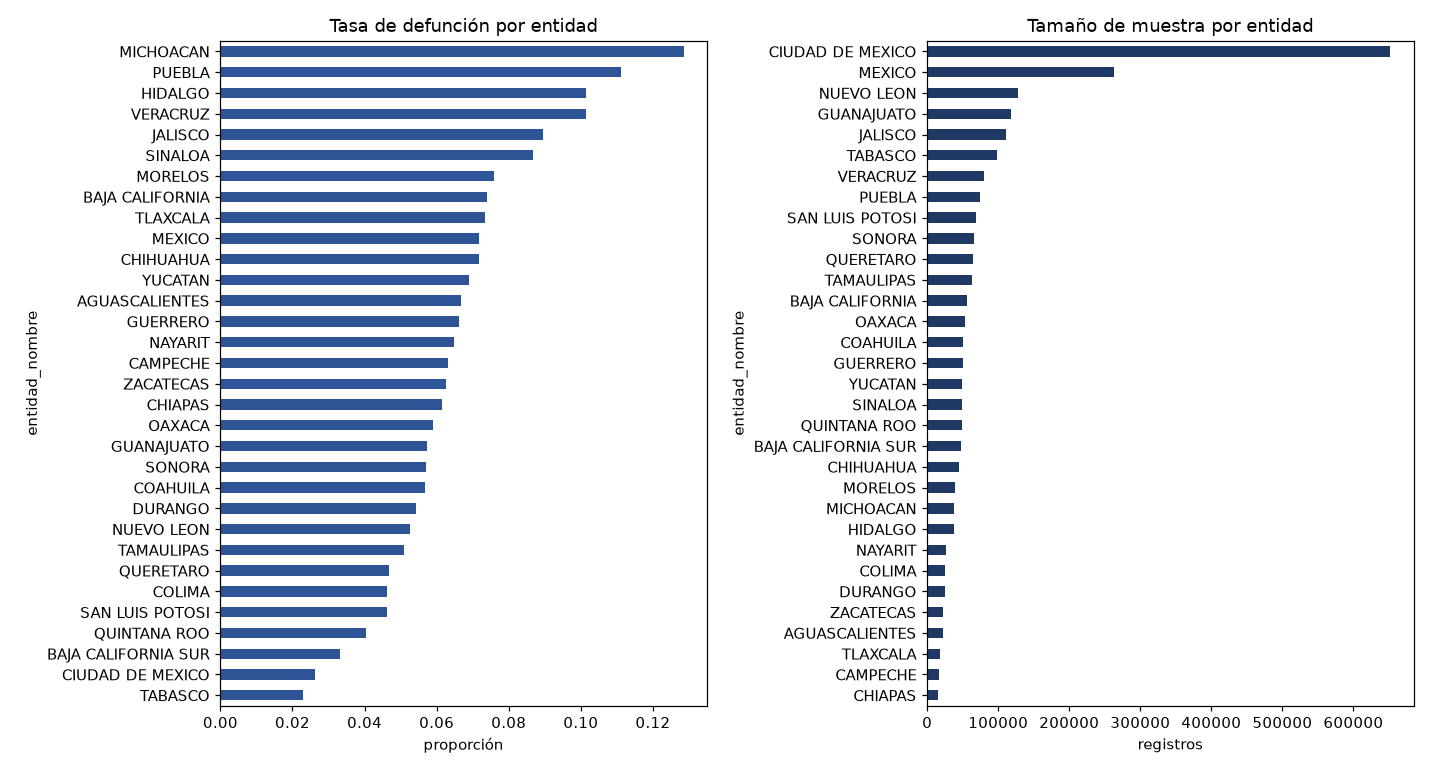
\includegraphics[width=\linewidth]{eda_por_entidad.png}
\caption{Heterogeneidad entre entidades federativas en la cohorte: tasa de
defunción (izquierda) y tamaño de muestra (derecha).}
\label{fig:eda}
\end{figure}

\section{Desempeño del modelo de referencia}

El modelo principal alcanza un \textbf{AUROC de \aurocGlobal} y un AUPRC de
\auprcGlobal{} sobre el conjunto de prueba ($n=\testN$), entrenado sobre
\nTrain{} registros y calibrado sobre \nCalib. La regresión logística
obtiene un AUROC de \logitAUROC, apenas por debajo, lo que indica que la señal
disponible en edad, sexo y comorbilidades es en buena medida lineal y que el
impulso del gradiente aporta poco en discriminación.

La comparación con la literatura sobre esta misma base debe hacerse con cautela,
porque los trabajos de referencia reportan exactitud y $F_1$ y no
AUROC~\parencite{becerra2022,mendez2024}, de modo que las cifras no son
directamente homologables. Lo que sí puede afirmarse es que el modelo no está
deliberadamente debilitado: usa los predictores habituales de esa literatura, un
algoritmo del mismo tipo y una cohorte de la misma fuente, y coincide con ella en
qué variables resultan más informativas (sección~\ref{sec:importancia}). Eso basta
para el propósito de la línea de base, que es que el sujeto de la auditoría sea un
modelo razonable y no un espantapájaros.

\subsection{Efecto de la calibración}

El modelo sin calibrar discrimina bien pero está severamente descalibrado: emite
un riesgo medio de \crudoRiesgo{} frente a una mortalidad observada de
\mortObsTest, es decir una sobreestimación por un factor de
\factorSobreestimacion, consecuencia directa de la reponderación por clase. La regresión isotónica ajustada sobre el
bloque de calibración reduce el puntaje de Brier de \brierCrudo{} a
\brierCalibrado{} y alinea el riesgo medio predicho (\calibRiesgo) con el
observado, dejando el AUROC esencialmente intacto --\aurocGlobal{} frente a
\crudoAUROC-- como corresponde a una transformación monótona.

\nota{Este resultado tiene una consecuencia que va más allá del ajuste. Una
auditoría de calibración por grupo realizada sobre el puntaje sin calibrar habría
reportado un error máximo de calibración por entidad de \errCalCrudo, cifra que
corresponde casi enteramente al sesgo global de entrenamiento y no a la inequidad
geográfica. Medida sobre el riesgo calibrado, la misma métrica es \errCalEntidad.
La conclusión sustantiva se invierte: la calibración por entidad, una vez
corregido el nivel global, es \emph{buena}.}

\subsection{Importancia de variables}
\label{sec:importancia}

La importancia por permutación sobre el AUROC (tabla~\ref{tab:importancia})
concentra la señal en dos variables: \texttt{\impPrimeraVar} (\impPrimera) y la
edad (\impSegunda). El resto de los predictores aporta \impTercera{} o menos cada
uno. La concentración es coherente con la literatura sobre esta
base~\parencite{becerra2022}, y refuerza la advertencia de la
sección~\ref{sec:fuga}: la validez del modelo depende de que la neumonía esté
efectivamente registrada al primer contacto.

% Generado por generar_tablas.py -- NO editar a mano.

\begin{table}[htbp]
\centering
\small
\caption{Importancia por permutación sobre el AUROC en el conjunto de prueba
(3 repeticiones, submuestra de \numprint{50000} observaciones).}
\label{tab:importancia}
\begin{tabular}{l r}
\toprule
Variable & Caída de AUROC \\
\midrule
NEUMONIA & 0.1057 \\
EDAD & 0.0789 \\
sexo\_mujer & 0.0029 \\
DIABETES & 0.0028 \\
RENAL\_CRONICA & 0.0016 \\
OBESIDAD & 0.0011 \\
OTRA\_COM & 0.0010 \\
HIPERTENSION & 0.0009 \\
INMUSUPR & 0.0002 \\
TABAQUISMO & 0.0001 \\
CARDIOVASCULAR & 0.0001 \\
EPOC & 0.0000 \\
ASMA & 0.0000 \\
\bottomrule
\end{tabular}
\end{table}


\section{Auditoría de equidad}

Todas las métricas dependientes de umbral se evalúan en el punto de operación
común $\tau=\umbralOperacion$, que alcanza una sensibilidad global de
\tprObjetivo{} con una tasa de falsos positivos de \fprObjetivo.

\subsection{Entidad federativa}

La tabla~\ref{tab:entidad} presenta el desempeño por entidad, la
tabla~\ref{tab:disparidad} resume las brechas por eje de auditoría y la
figura~\ref{fig:equidad} las visualiza. El hallazgo
central es una \textbf{disparidad geográfica sustantiva}: la sensibilidad varía
\gapTPRentidad{} entre entidades y el AUROC \gapAUROCentidad. El peor desempeño
corresponde a \entPeor{} (AUROC \entPeorAUROC, sensibilidad \entPeorTPR) y el
mejor a \entMejor{} (AUROC \entMejorAUROC, sensibilidad \entMejorTPR).

La magnitud merece leerse en términos clínicos y no estadísticos. Con un umbral
único calibrado para detectar al \sensObjetivo\,\% de las defunciones a nivel
nacional, el modelo detecta cerca de \entPeorPct{} de cada 100 en la entidad peor
servida y \entMejorPct{} de cada 100 en la mejor servida. La diferencia --unas
\entDifPct{} defunciones no priorizadas por cada 100-- recae sobre la población de un estado concreto por el solo hecho de residir
en él.

% Generado por generar_tablas.py -- NO editar a mano.

\begin{table}[htbp]
\centering
\caption{Brechas máximas entre grupos por eje de auditoría, al umbral
$\tau=0.1562$. La brecha de TPR corresponde a la violación de
\emph{equalized odds}; el error de calibración se mide sobre el riesgo calibrado.}
\label{tab:disparidad}
\small\setlength{\tabcolsep}{5pt}
\begin{tabular}{l r r r r r}
\toprule
Eje & $\Delta$TPR & $\Delta$FPR & $\Delta$AUROC & $\Delta$Selec. & Err.\ calib. \\
\midrule
Entidad federativa & 0.2935 & 0.0867 & 0.0563 & 0.1556 & 0.0231 \\
Sexo & 0.0393 & 0.0268 & 0.0082 & 0.0448 & 0.0005 \\
Grupo etario & 0.5824 & 0.3026 & 0.0903 & 0.4408 & 0.0008 \\
\bottomrule
\end{tabular}
\end{table}

% Generado por generar_tablas.py -- NO editar a mano.

\begingroup
\small\setlength{\tabcolsep}{4pt}
\begin{longtable}{l r r r r r r}
\caption{Desempeño y equidad por entidad federativa en el conjunto de prueba
($n=631\,663$), al umbral de sensibilidad objetivo
$\tau=0.1562$. Ordenadas por AUROC ascendente.}
\label{tab:entidad}\\
\toprule
Entidad & $n$ & Mort. & AUROC & TPR & FPR & Riesgo \\
\midrule
\endfirsthead
\toprule
Entidad & $n$ & Mort. & AUROC & TPR & FPR & Riesgo \\
\midrule
\endhead
\midrule
\multicolumn{7}{r}{\footnotesize Continúa en la página siguiente} \\
\endfoot
\bottomrule
\endlastfoot
Chihuahua & 11\,072 & 0.0713 & 0.9207 & 0.688 & 0.081 & 0.0659 \\
Chiapas & 3\,831 & 0.0611 & 0.9265 & 0.662 & 0.065 & 0.0567 \\
Baja California Sur & 11\,712 & 0.0307 & 0.9272 & 0.683 & 0.040 & 0.0347 \\
Aguascalientes & 5\,498 & 0.0615 & 0.9304 & 0.657 & 0.060 & 0.0532 \\
Durango & 6\,297 & 0.0569 & 0.9310 & 0.631 & 0.052 & 0.0465 \\
Veracruz & 20\,275 & 0.1012 & 0.9340 & 0.766 & 0.086 & 0.0826 \\
Nuevo León & 32\,110 & 0.0528 & 0.9341 & 0.686 & 0.046 & 0.0449 \\
Coahuila & 12\,615 & 0.0576 & 0.9342 & 0.686 & 0.054 & 0.0502 \\
Jalisco & 27\,918 & 0.0887 & 0.9348 & 0.703 & 0.067 & 0.0656 \\
Michoacán & 9\,484 & 0.1281 & 0.9359 & 0.853 & 0.116 & 0.1114 \\
México & 65\,705 & 0.0720 & 0.9387 & 0.760 & 0.070 & 0.0634 \\
Tlaxcala & 4\,288 & 0.0702 & 0.9391 & 0.841 & 0.100 & 0.0780 \\
Sinaloa & 12\,274 & 0.0849 & 0.9394 & 0.799 & 0.076 & 0.0735 \\
Nayarit & 6\,700 & 0.0710 & 0.9402 & 0.700 & 0.049 & 0.0537 \\
Hidalgo & 9\,345 & 0.1022 & 0.9410 & 0.881 & 0.123 & 0.1011 \\
Zacatecas & 5\,534 & 0.0614 & 0.9431 & 0.773 & 0.067 & 0.0591 \\
Yucatán & 12\,490 & 0.0705 & 0.9440 & 0.726 & 0.048 & 0.0515 \\
Puebla & 18\,800 & 0.1130 & 0.9480 & 0.920 & 0.118 & 0.1083 \\
Oaxaca & 13\,461 & 0.0558 & 0.9512 & 0.792 & 0.060 & 0.0560 \\
Querétaro & 16\,305 & 0.0449 & 0.9530 & 0.816 & 0.055 & 0.0497 \\
Tamaulipas & 15\,876 & 0.0544 & 0.9539 & 0.809 & 0.048 & 0.0509 \\
Campeche & 4\,191 & 0.0625 & 0.9544 & 0.920 & 0.111 & 0.0837 \\
Guanajuato & 29\,653 & 0.0575 & 0.9579 & 0.833 & 0.061 & 0.0586 \\
Baja California & 13\,953 & 0.0754 & 0.9584 & 0.887 & 0.080 & 0.0782 \\
Colima & 6\,390 & 0.0444 & 0.9598 & 0.824 & 0.052 & 0.0496 \\
Morelos & 9\,756 & 0.0763 & 0.9600 & 0.914 & 0.095 & 0.0875 \\
Ciudad de México & 162\,746 & 0.0262 & 0.9607 & 0.808 & 0.040 & 0.0367 \\
Quintana Roo & 12\,151 & 0.0414 & 0.9623 & 0.813 & 0.041 & 0.0393 \\
Sonora & 16\,698 & 0.0562 & 0.9628 & 0.868 & 0.064 & 0.0621 \\
San Luis Potosí & 17\,326 & 0.0459 & 0.9647 & 0.868 & 0.057 & 0.0528 \\
Guerrero & 12\,589 & 0.0666 & 0.9679 & 0.925 & 0.080 & 0.0751 \\
Tabasco & 24\,620 & 0.0222 & 0.9770 & 0.879 & 0.036 & 0.0348 \\
\end{longtable}
\endgroup


\begin{figure}[htbp]
\centering
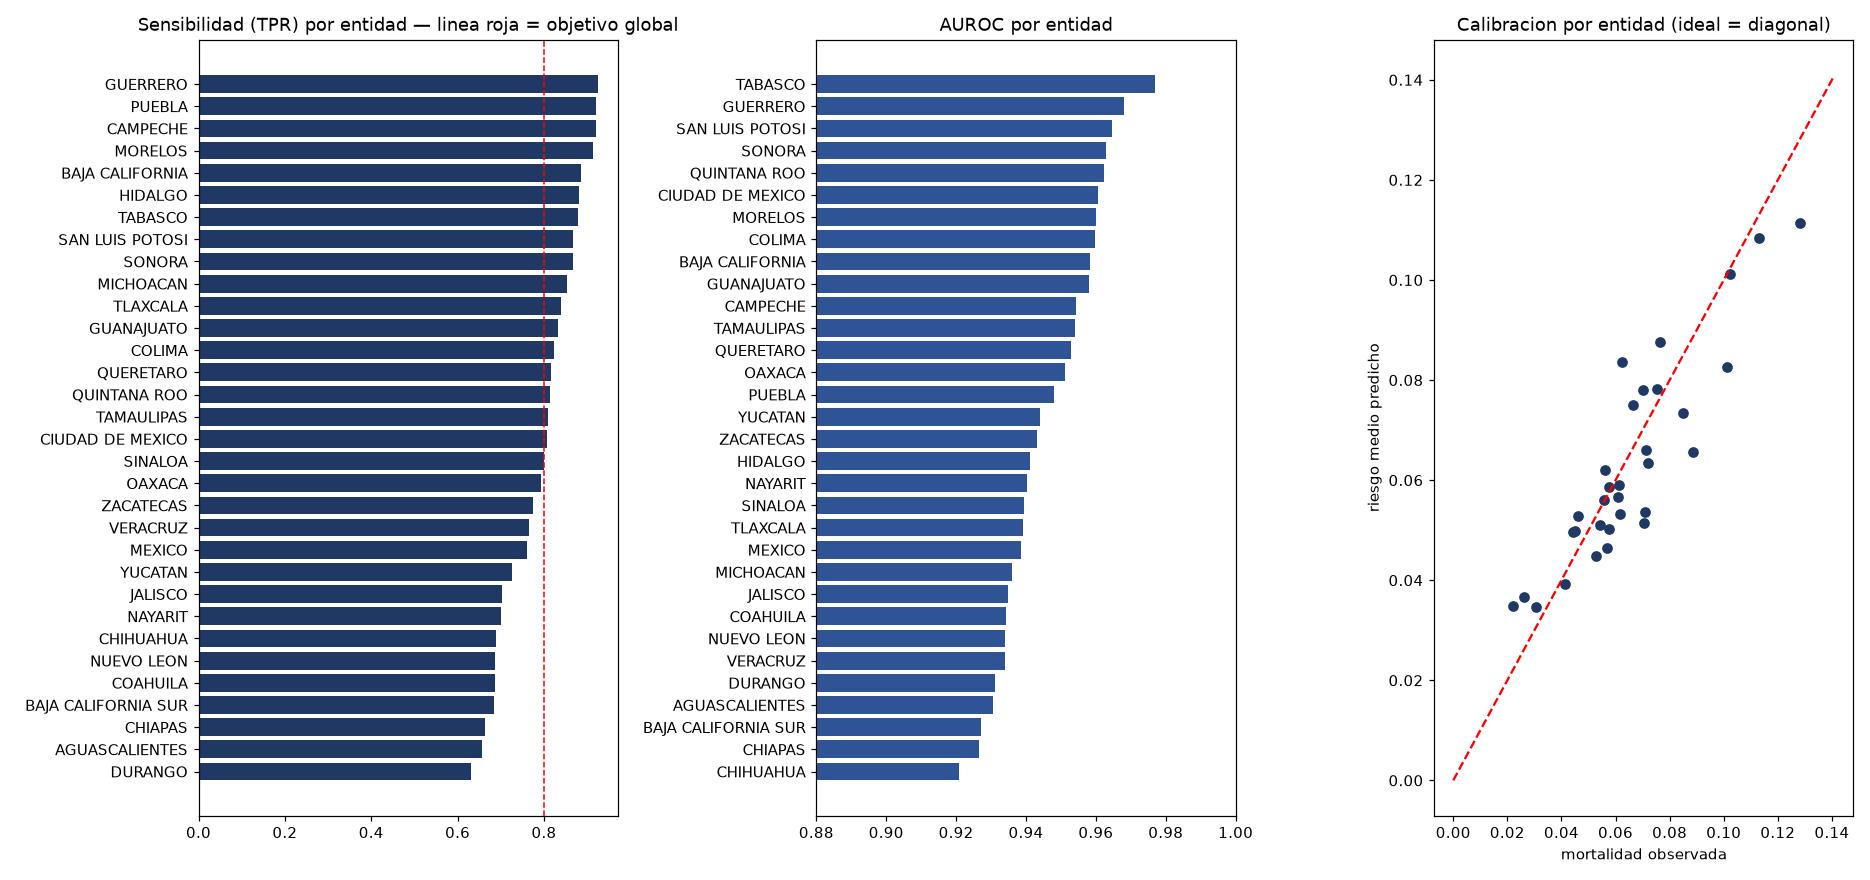
\includegraphics[width=\linewidth]{equidad_por_entidad.png}
\caption{Auditoría por entidad federativa: sensibilidad frente al objetivo global
(izquierda), AUROC (centro) y calibración, riesgo medio predicho frente a
mortalidad observada (derecha).}
\label{fig:equidad}
\end{figure}

Conviene notar la disociación entre criterios de equidad. El error máximo de
calibración por entidad es \errCalEntidad, es decir, la probabilidad emitida
significa aproximadamente lo mismo en cada estado; sin embargo la brecha de
sensibilidad es \gapTPRentidad. Un modelo puede estar bien calibrado en todos los
grupos y repartir la sensibilidad de forma muy desigual: es exactamente el
comportamiento que anticipa el teorema de imposibilidad cuando las prevalencias
difieren entre grupos~\parencite{chouldechova2017,kleinberg2017}. Conviene
subrayar que la calibración es propiedad del puntaje y no de la regla de
decisión, de modo que el error de \errCalEntidad{} no se altera por ninguna
elección de umbral, incluida la mitigación de la
sección~\ref{sec:mitigacion_res}. El mecanismo es
directo: con un umbral fijo sobre un puntaje bien calibrado, la fracción de
positivos que quedan por encima del corte depende de la distribución de riesgo
dentro del grupo, y esa distribución es distinta en cada entidad.

\subsection{Incertidumbre de las brechas}
\label{sec:incertidumbre_res}

Las cifras anteriores son estimaciones puntuales sobre un único conjunto de
prueba. La tabla~\ref{tab:incertidumbre} añade intervalos de confianza al
95\,\% por remuestreo y la tabla~\ref{tab:permutacion} contrasta las brechas
contra su distribución bajo la hipótesis nula de que la entidad no influye
(sección~\ref{sec:incertidumbre}).

% Generado por generar_tablas.py -- NO editar a mano.

\begin{table}[htbp]
\centering
\small\setlength{\tabcolsep}{4pt}
\caption{Desempeño por entidad con intervalos de confianza al 95\,\% obtenidos
por remuestreo estratificado (1000 réplicas); cinco peores y cinco
mejores por AUROC.}
\label{tab:incertidumbre}
\begin{tabular}{l r r c r c}
\toprule
Entidad & $n$ & AUROC & IC 95\,\% & TPR & IC 95\,\% \\
\midrule
Chihuahua & 11\,072 & 0.9207 & [0.9125,\,0.9290] & 0.688 & [0.654,\,0.720] \\
Chiapas & 3\,831 & 0.9265 & [0.9116,\,0.9407] & 0.662 & [0.604,\,0.721] \\
Baja California Sur & 11\,712 & 0.9272 & [0.9135,\,0.9398] & 0.683 & [0.635,\,0.731] \\
Aguascalientes & 5\,498 & 0.9304 & [0.9182,\,0.9418] & 0.657 & [0.603,\,0.705] \\
Durango & 6\,297 & 0.9310 & [0.9190,\,0.9427] & 0.631 & [0.580,\,0.680] \\
\midrule
Quintana Roo & 12\,151 & 0.9623 & [0.9539,\,0.9699] & 0.813 & [0.777,\,0.845] \\
Sonora & 16\,698 & 0.9628 & [0.9582,\,0.9677] & 0.868 & [0.847,\,0.889] \\
San Luis Potosí & 17\,326 & 0.9647 & [0.9587,\,0.9701] & 0.868 & [0.844,\,0.891] \\
Guerrero & 12\,589 & 0.9679 & [0.9635,\,0.9720] & 0.925 & [0.907,\,0.943] \\
Tabasco & 24\,620 & 0.9770 & [0.9717,\,0.9820] & 0.879 & [0.851,\,0.907] \\
\bottomrule
\end{tabular}
\end{table}

% Generado por generar_tablas.py -- NO editar a mano.

\begin{table}[htbp]
\centering
\small
\caption{Prueba de permutación sobre las brechas entre entidades
(1000 permutaciones de las etiquetas de entidad, conservando
los tamaños de grupo). La brecha bajo la nula no es cero: con 32 grupos, máximo y
mínimo se separan por azar.}
\label{tab:permutacion}
\begin{tabular}{l r r r r}
\toprule
Brecha & Observada & IC 95\,\% & Nula (mediana) & $p$ \\
\midrule
AUROC & 0.0563 & [0.0496,\,0.0697] & 0.0175 & 0.001 \\
Sensibilidad & 0.2935 & [0.2671,\,0.3535] & 0.0737 & 0.001 \\
\bottomrule
\end{tabular}
\end{table}


\begin{figure}[htbp]
\centering
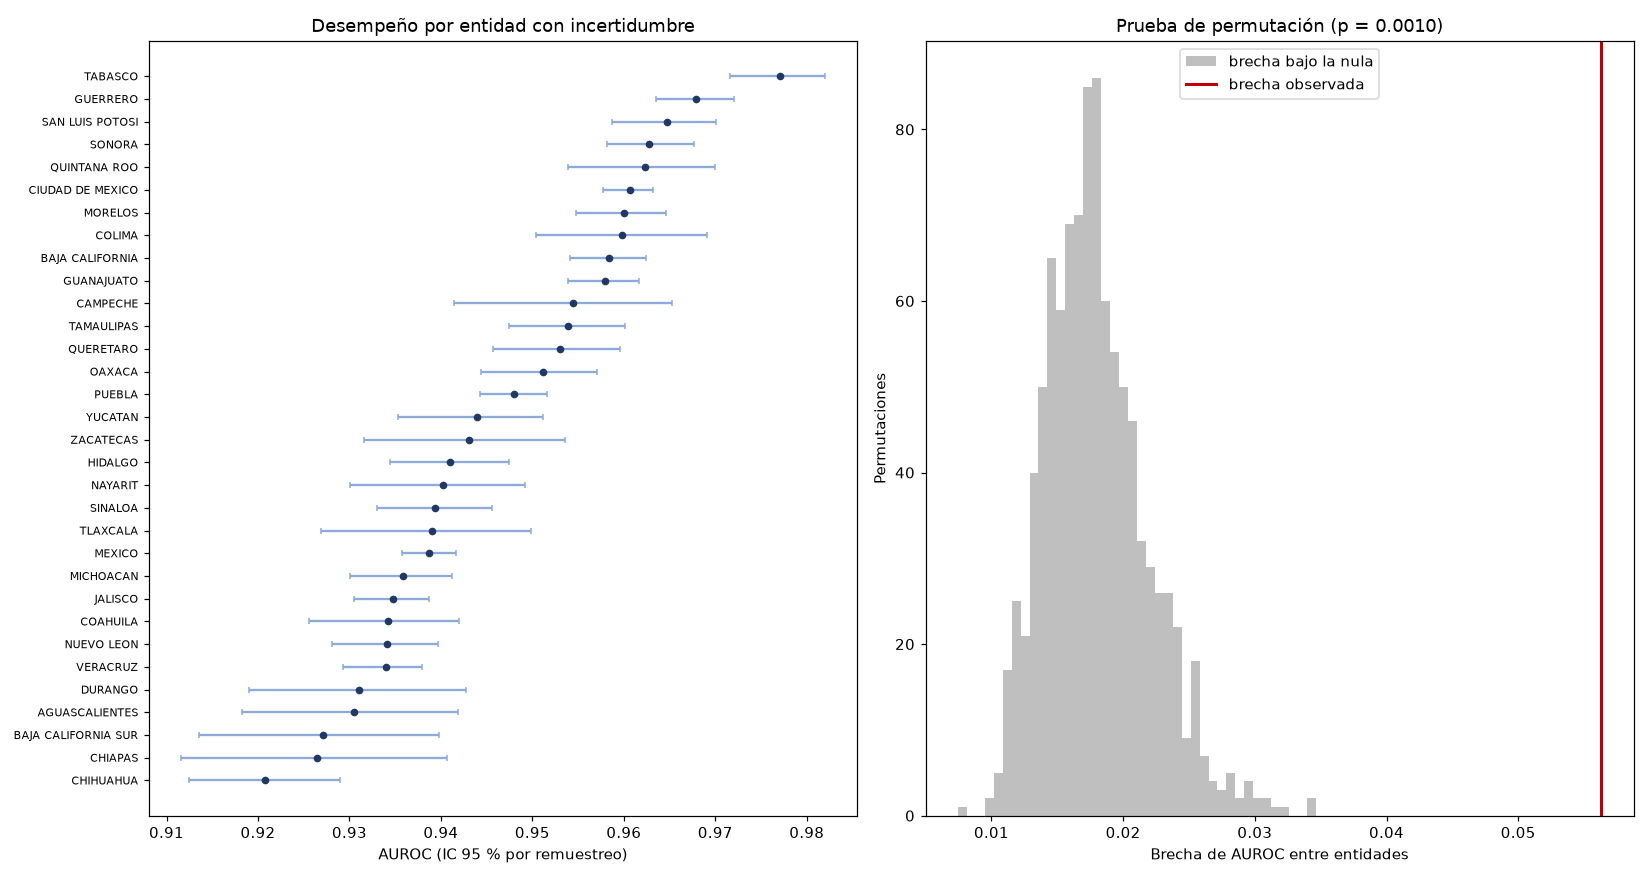
\includegraphics[width=\linewidth]{incertidumbre_brechas.png}
\caption{Izquierda: AUROC por entidad con intervalo de confianza al 95\,\%.
Derecha: distribución de la brecha de AUROC bajo la hipótesis nula de ausencia de
efecto de entidad, frente a la brecha observada.}
\label{fig:incertidumbre}
\end{figure}

El resultado más importante es que \textbf{las brechas bajo la nula no son cero}.
Permutando al azar las etiquetas de entidad, la brecha mediana de AUROC es
\nulaAuroc{} y la de sensibilidad \nulaTpr: con 32 grupos de tamaños desiguales,
el máximo y el mínimo se separan por azar sin que haya efecto alguno. Ese es el
punto de comparación correcto, y no el cero.

Contra esa referencia, las brechas observadas son claramente excesivas. La de
AUROC, \gapAUROCentidad{} (IC 95\,\%: \gapAurocICa--\gapAurocICb), supera el
percentil 95 de la nula (\nulaAurocPsup); la de sensibilidad, \gapTPRentidad{}
(IC 95\,\%: \gapTprICa--\gapTprICb), supera con holgura el suyo (\nulaTprPsup). En
ambos casos $p=\pAuroc$ y $p=\pTpr$ respectivamente, que es el mínimo alcanzable
con \boP{} permutaciones: ninguna reasignación al azar produjo una brecha tan
grande como la real.

Conviene traducir esto a la magnitud del efecto. De la brecha de sensibilidad
observada, alrededor de \nulaTpr{} es lo que el azar produce con esta estructura
de grupos; el exceso atribuible a la entidad es de aproximadamente \excesoTpr.
Sigue siendo grande, pero es la cifra honesta.

A nivel de entidad individual, \paresDisjuntos{} de los \paresTotal{} pares
posibles tienen intervalos de AUROC disjuntos (\paresPct\,\%), y los extremos
--\entPeor{} y \entMejor-- lo están. La precisión es razonable incluso en las
entidades pequeñas: el intervalo más ancho es el de \icAncho{} ($n=\icAnchoN$),
con una amplitud de \icAnchoAmp. El ordenamiento fino de la
tabla~\ref{tab:entidad} no debe leerse posición por posición, pero la separación
entre los extremos no es ruido.

\subsection{Sexo y grupo etario}

Las tablas~\ref{tab:sexo} y~\ref{tab:edad} presentan los otros dos ejes. El sesgo
por \textbf{sexo} es pequeño: la brecha de sensibilidad es \gapTPRsexo{} y la de
AUROC \gapAUROCsexo. El sesgo por \textbf{grupo etario} es el mayor de los tres
--brecha de sensibilidad \gapTPRedad{} y de AUROC \gapAUROCedad-- pero su
interpretación es distinta.

% Generado por generar_tablas.py -- NO editar a mano.

\begin{table}[htbp]
\centering
\small\setlength{\tabcolsep}{4pt}
\caption{Desempeño y equidad por sexo en el conjunto de prueba.}
\label{tab:sexo}
\begin{tabular}{l r r r r r r r}
\toprule
Sexo & $n$ & Mort. & AUROC & TPR & FPR & Selec. & Riesgo \\
\midrule
Hombre & 309\,437 & 0.0681 & 0.9456 & 0.811 & 0.073 & 0.123 & 0.0676 \\
Mujer & 322\,226 & 0.0444 & 0.9538 & 0.772 & 0.046 & 0.079 & 0.0444 \\
\bottomrule
\end{tabular}
\end{table}

% Generado por generar_tablas.py -- NO editar a mano.

\begin{table}[htbp]
\centering
\small\setlength{\tabcolsep}{4pt}
\caption{Desempeño y equidad por grupo etario en el conjunto de prueba.}
\label{tab:edad}
\begin{tabular}{l r r r r r r r}
\toprule
Grupo etario & $n$ & Mort. & AUROC & TPR & FPR & Selec. & Riesgo \\
\midrule
0-17 & 47\,676 & 0.0029 & 0.9347 & 0.266 & 0.003 & 0.004 & 0.0027 \\
18-39 & 303\,100 & 0.0089 & 0.9346 & 0.608 & 0.015 & 0.020 & 0.0089 \\
40-59 & 196\,593 & 0.0558 & 0.9039 & 0.743 & 0.062 & 0.100 & 0.0554 \\
60+ & 84\,285 & 0.2560 & 0.8444 & 0.849 & 0.306 & 0.445 & 0.2552 \\
\bottomrule
\end{tabular}
\end{table}


La brecha etaria es en buena medida mecánica y no debe leerse como inequidad en el
mismo sentido. La edad es el segundo predictor más informativo y las tasas base
difieren por dos órdenes de magnitud: \edadMenorTasa\,\% en menores de 18 años
frente a \edadMayorTasa\,\% en el grupo de 60 o más. Con un umbral único sobre un puntaje calibrado,
un grupo con riesgo basal muy bajo cae casi enteramente por debajo del corte, y su
sensibilidad se hunde por construcción: en 0--17 años es \edadMenorTPR{} con una
tasa de selección de \edadMenorSel\,\%. Igualar la sensibilidad entre grupos etarios exigiría
seleccionar una fracción mucho mayor de menores, con un valor predictivo positivo
muy bajo, algo difícil de justificar clínicamente. La disparidad geográfica no
admite esa explicación, porque las entidades no difieren en riesgo basal de forma
comparable ni la entidad es un predictor del modelo.

\subsection{Análisis interseccional}
\label{sec:interseccional}

Para descartar que la brecha geográfica sea un reflejo de la composición etaria de
cada estado, se repite la auditoría restringiendo la muestra a adultos de
\textbf{60 años o más} (tabla~\ref{tab:interseccional}). La disparidad no
desaparece: el AUROC varía de \sesentaPeorAUROC{} en \sesentaPeor{} a
\sesentaMejorAUROC{} en \sesentaMejor, un rango de \sesentaRango{} frente a
\gapAUROCentidad{} en la población completa.

% Generado por generar_tablas.py -- NO editar a mano.

\begin{table}[htbp]
\centering
\caption{Subgrupo interseccional: adultos de 60 años o más, por entidad
(cinco peores y cinco mejores de 32 evaluadas). El deterioro persiste
tras controlar por edad avanzada.}
\label{tab:interseccional}
\begin{tabular}{l r r r r}
\toprule
Entidad & $n$ & Mortalidad & AUROC & TPR \\
\midrule
Chiapas & 482 & 0.322 & 0.688 & 0.748 \\
Chihuahua & 1\,798 & 0.274 & 0.737 & 0.732 \\
Jalisco & 4\,212 & 0.382 & 0.758 & 0.771 \\
Aguascalientes & 730 & 0.311 & 0.763 & 0.771 \\
Veracruz & 3\,243 & 0.385 & 0.764 & 0.792 \\
\midrule
Campeche & 599 & 0.295 & 0.881 & 0.977 \\
San Luis Potosí & 2\,495 & 0.202 & 0.889 & 0.897 \\
Guerrero & 2\,046 & 0.277 & 0.889 & 0.951 \\
Ciudad de México & 20\,942 & 0.128 & 0.895 & 0.858 \\
Tabasco & 2\,801 & 0.117 & 0.942 & 0.930 \\
\bottomrule
\end{tabular}
\end{table}


Este es el resultado más consistente con la hipótesis~\ref{h1} en su formulación
fuerte: la inequidad geográfica es una propiedad del modelo y no un artefacto de
la estructura demográfica de las entidades.

Dos matices impiden sobreinterpretarlo. El primero es de precisión: los subgrupos
son pequeños --\sesentaPeor{} aporta apenas \sesentaPeorN{} observaciones-- de
modo que buena parte de la amplitud del rango es varianza de muestreo y no
inequidad estimada con fiabilidad. Los intervalos de confianza de la
sección~\ref{sec:incertidumbre_res} se calcularon sobre la población completa, no
dentro de este subgrupo, donde los tamaños son un orden de magnitud menores; para
él sigue sin haber una medida de precisión.

De hecho \sesentaPeor{} queda por debajo del criterio general de soporte, que se
relajó aquí a \interMinN{} observaciones (sección~\ref{sec:particion}). Aplicando
el criterio de \numprint{500} quedarían \interNestandar{} entidades, el peor
desempeño sería \interPeorEstandar{} con \interPeorEstandarAUROC{} y el rango
bajaría a \interRangoEstandar. La conclusión no depende de la elección: bajo
cualquiera de los dos criterios la dispersión dentro del subgrupo supera con
holgura la de la población completa (\gapAUROCentidad).

El segundo es que la ampliación del rango de AUROC dentro de los adultos mayores
matiza el diagnóstico de la sección~\ref{sec:mitigacion_res}. En la población
completa la disparidad reside claramente en el umbral y no en el ordenamiento;
dentro del subgrupo de 60 años o más, en cambio, la dispersión del AUROC es del
mismo orden que la de la sensibilidad, lo que sugiere que ahí también hay un
componente de ordenamiento. Si es así, una mitigación basada solo en umbrales
sería menos efectiva en ese subgrupo que en la población general. Comprobarlo
exige repetir la mitigación dentro del subgrupo, algo que este trabajo no hace.

Conviene además no leer el resultado en clave de marginación. El subgrupo con
peor discriminación (\sesentaPeor, grado «Muy alto») no es el de mayor mortalidad
--esa es \sesentaMasLetal, con \sesentaMasLetalTasa{} frente a
\sesentaPeorTasa-- y entre los cinco mejores figura Guerrero, la entidad con
mayor marginación del país. El patrón por grado de marginación se examina en la
sección~\ref{sec:correlatos} y no aparece.

\subsection{Correlatos de la inequidad geográfica}
\label{sec:correlatos}

Se examinó la asociación entre el desempeño por entidad y tres características
del grupo. Sobre las \nEntidades{} entidades:

\begin{itemize}[leftmargin=*]
  \item \textbf{Tamaño de muestra.} $r=\corrAurocNr$ ($p=\corrAurocNp$);
    Spearman $\rho=\corrAurocNrho$ ($p=\corrAurocNprho$). Asociación positiva
    débil y no significativa.
  \item \textbf{Tasa de mortalidad de la entidad.} $r=\corrAurocTasar$
    ($p=\corrAurocTasap$); $\rho=\corrAurocTasarho$ ($p=\corrAurocTasaprho$).
    Es la única asociación que alcanza significación convencional: el modelo
    discrimina peor en las entidades con mayor mortalidad observada.
  \item \textbf{Índice de marginación.} $r=\corrMargAurocr$
    ($p=\corrMargAurocp$); $\rho=\corrMargAurocrho$ ($p=\corrMargAurocprho$).
    Sin asociación detectable. Para la sensibilidad, $r=\corrMargTprr$
    ($p=\corrMargTprp$).
\end{itemize}

El índice de marginación procede del archivo por entidad de los \emph{Índices de
marginación 2020} de CONAPO, construidos sobre el Censo de Población y Vivienda
2020~\parencite{conapo2020}. Conviene precisar su escala, porque se presta a
confusión: la edición 2020 se calcula por Distancias Ponderadas al cuadrado y un
valor \emph{más alto} indica \emph{menor} marginación --Guerrero 10.99, grado
«Muy alto»; Nuevo León 23.44, grado «Muy bajo»--. El «índice normalizado» acotado
a $[0,1]$ pertenece a las ediciones anteriores, basadas en componentes
principales, y su dirección es la contraria.

Como una correlación lineal puede ocultar un patrón escalonado, y el grado es la
forma en que CONAPO comunica el índice, la tabla~\ref{tab:marginacion} agrega el
desempeño por grado de marginación. No aparece gradiente alguno: el AUROC medio
oscila entre \gradoAurocMin{} y \gradoAurocMax{} sin orden discernible, y una
prueba de Kruskal--Wallis entre grados no detecta diferencia ($H=\kruskalH$,
$p=\kruskalP$). Llama la atención que el grupo con menor AUROC medio sea el de
marginación \emph{\gradoPeor}, lo contrario de lo que anticipaba la
hipótesis~\ref{h2}.

% Generado por generar_tablas.py -- NO editar a mano.

\begin{table}[htbp]
\centering
\small
\caption{Desempeño medio por grado de marginación (CONAPO 2020), de mayor a
menor carencia. Kruskal--Wallis sobre el AUROC entre grados:
$H=1.827$, $p=0.768$.}
\label{tab:marginacion}
\begin{tabular}{l r r r}
\toprule
Grado de marginación & Entidades & AUROC medio & TPR medio \\
\midrule
Muy alto & 3 & 0.9485 & 0.793 \\
Alto & 9 & 0.9451 & 0.808 \\
Medio & 8 & 0.9484 & 0.816 \\
Bajo & 8 & 0.9486 & 0.794 \\
Muy bajo & 4 & 0.9399 & 0.709 \\
\bottomrule
\end{tabular}
\end{table}


\section{Sensibilidad: la población en la que el desenlace es posible}
\label{sec:sensibilidad_res}

Como se declaró en la sección~\ref{sec:fuga}, en esta cohorte fallecer implica
estar registrado como hospitalizado. El modelo separa \defTotales{}
defunciones de un conjunto de supervivientes del que la gran mayoría son casos
ambulatorios que no pueden fallecer. La tabla~\ref{tab:sensibilidad} compara la
cohorte completa con el subconjunto hospitalizado, que es la población en riesgo.

% Generado por generar_tablas.py -- NO editar a mano.

\begin{table}[htbp]
\centering
\small
\caption{Análisis de sensibilidad: cohorte completa frente al subconjunto
hospitalizado, que es donde el desenlace es posible. El AUPRC se acompaña de su
razón respecto de la prevalencia, que es su línea base.}
\label{tab:sensibilidad}
\begin{tabular}{l r r}
\toprule
& Cohorte completa & Solo hospitalizados \\
\midrule
$n$ & 2\,526\,649 & 297\,685 \\
Prevalencia del desenlace & 0.056 & 0.475 \\
\midrule
AUROC & 0.9503 & 0.7001 \\
AUPRC & 0.5533 & 0.6370 \\
AUPRC / prevalencia & 9.88$\times$ & 1.34$\times$ \\
Brier & 0.0323 & 0.2179 \\
\midrule
$\Delta$TPR entre entidades & 0.2935 & 0.1876 \\
$\Delta$AUROC entre entidades & 0.0563 & 0.1494 \\
\bottomrule
\end{tabular}
\end{table}


El contraste es grande y hay que enunciarlo sin rodeos: el AUROC pasa de
\aurocGlobal{} a \hospAUROC. Buena parte de la discriminación de la cohorte
completa consiste en separar ambulatorios de hospitalizados, tarea que
\texttt{\impPrimeraVar} al primer contacto resuelve muy bien --lo que explica que
domine la importancia por encima de la edad, algo anómalo en un modelo de
mortalidad por COVID.

El AUPRC ilustra el mismo punto y advierte contra una lectura ingenua: sube de
\auprcGlobal{} a \hospAUPRC, pero su línea base es la prevalencia, que pasa de
\cohorteTasaDef\,\% a \hospPrev. Normalizado, el poder discriminante cae de
\completaLift$\times$ la prevalencia a \hospLift$\times$: un AUPRC mayor sobre una
señal mucho más débil.

Nada de esto invalida la cohorte principal, que responde a una pregunta legítima
--priorizar al primer contacto entre todos los casos confirmados-- pero sí fija
con qué puede compararse cada cifra. El \aurocGlobal{} no es homologable a un
modelo de mortalidad hospitalaria; el \hospAUROC{} sí.

\subsection{Efecto sobre el diagnóstico de equidad}

Lo relevante para esta tesis es que la estructura del sesgo cambia. En la
población en riesgo la brecha de sensibilidad \emph{baja} de \gapTPRentidad{} a
\hospGapTPR, mientras la de AUROC casi se triplica, de \gapAUROCentidad{} a
\hospGapAUROC{} --con \hospPeor{} en \hospPeorAUROC{} y \hospMejor{} en
\hospMejorAUROC.

Es decir: la disparidad se desplaza del umbral hacia el ordenamiento. El
diagnóstico de la sección~\ref{sec:mitigacion_res} --que el problema está en
dónde se corta y no en cómo se ordena-- vale para la cohorte completa, pero se
invierte parcialmente entre los pacientes hospitalizados. Es el mismo patrón que
apareció en el subgrupo de 60 años o más, y con la misma consecuencia práctica:
la mitigación por umbrales, que es la que funciona en la cohorte completa, sería
menos suficiente en la población clínicamente crítica.

\subsection{¿Depende el resultado de una sola variable?}

La sección~\ref{sec:importancia} mostró que \texttt{\impPrimeraVar} concentra la
importancia, y la sección~\ref{sec:fuga} advirtió que su validez descansa en un
supuesto sobre la práctica de registro. Si la inequidad geográfica fuera un
artefacto de que unos estados registran neumonía mejor que otros, debería
desaparecer al quitar esa variable.

No desaparece. Reentrenando con los \sinNeuNpred{} predictores restantes, el
AUROC baja de \aurocGlobal{} a \sinNeuAUROC{} --una caída de \sinNeuCaida, que
confirma su peso-- y el AUPRC cae de \auprcGlobal{} a \sinNeuAUPRC. Pero la
disparidad persiste: la brecha de AUROC entre entidades es \sinNeuGapAUROC,
ligeramente \emph{mayor} que la de \gapAUROCentidad{} del modelo completo, y la
de sensibilidad baja a \sinNeuGapTPR{} sin acercarse a desaparecer.

La inequidad geográfica no es, por tanto, un efecto de la práctica de registro de
esa variable. Sobrevive a un modelo que no la usa, y con la brecha de
discriminación incluso algo más amplia.

\section{Transportabilidad geográfica interna}
\label{sec:loeo_res}

Los resultados anteriores evalúan el modelo en entidades que participaron en su
entrenamiento. La tabla~\ref{tab:loeo} y la figura~\ref{fig:loeo} muestran qué
ocurre cuando la entidad evaluada fue excluida por completo
(sección~\ref{sec:loeo}).

% Generado por generar_tablas.py -- NO editar a mano.

\begin{table}[htbp]
\centering
\small
\caption{Transportabilidad geográfica interna: AUROC de cada entidad cuando
participó en el entrenamiento frente a cuando fue excluida por completo (seis
mayores pérdidas y cuatro mayores ganancias de 32 entidades).}
\label{tab:loeo}
\begin{tabular}{l r r r r}
\toprule
Entidad & $n$ & AUROC interno & AUROC no vista & $\Delta$ \\
\midrule
Tlaxcala & 17\,431 & 0.9391 & 0.9283 & -0.0108 \\
Michoacán & 38\,126 & 0.9359 & 0.9280 & -0.0079 \\
Morelos & 39\,258 & 0.9600 & 0.9552 & -0.0048 \\
Puebla & 75\,074 & 0.9480 & 0.9435 & -0.0045 \\
Colima & 25\,536 & 0.9598 & 0.9558 & -0.0040 \\
Guanajuato & 118\,324 & 0.9579 & 0.9539 & -0.0040 \\
\midrule
Yucatán & 49\,748 & 0.9440 & 0.9480 & +0.0040 \\
Tamaulipas & 63\,741 & 0.9539 & 0.9592 & +0.0053 \\
Campeche & 16\,881 & 0.9544 & 0.9601 & +0.0057 \\
Durango & 25\,123 & 0.9310 & 0.9376 & +0.0066 \\
\bottomrule
\end{tabular}
\end{table}


\begin{figure}[htbp]
\centering
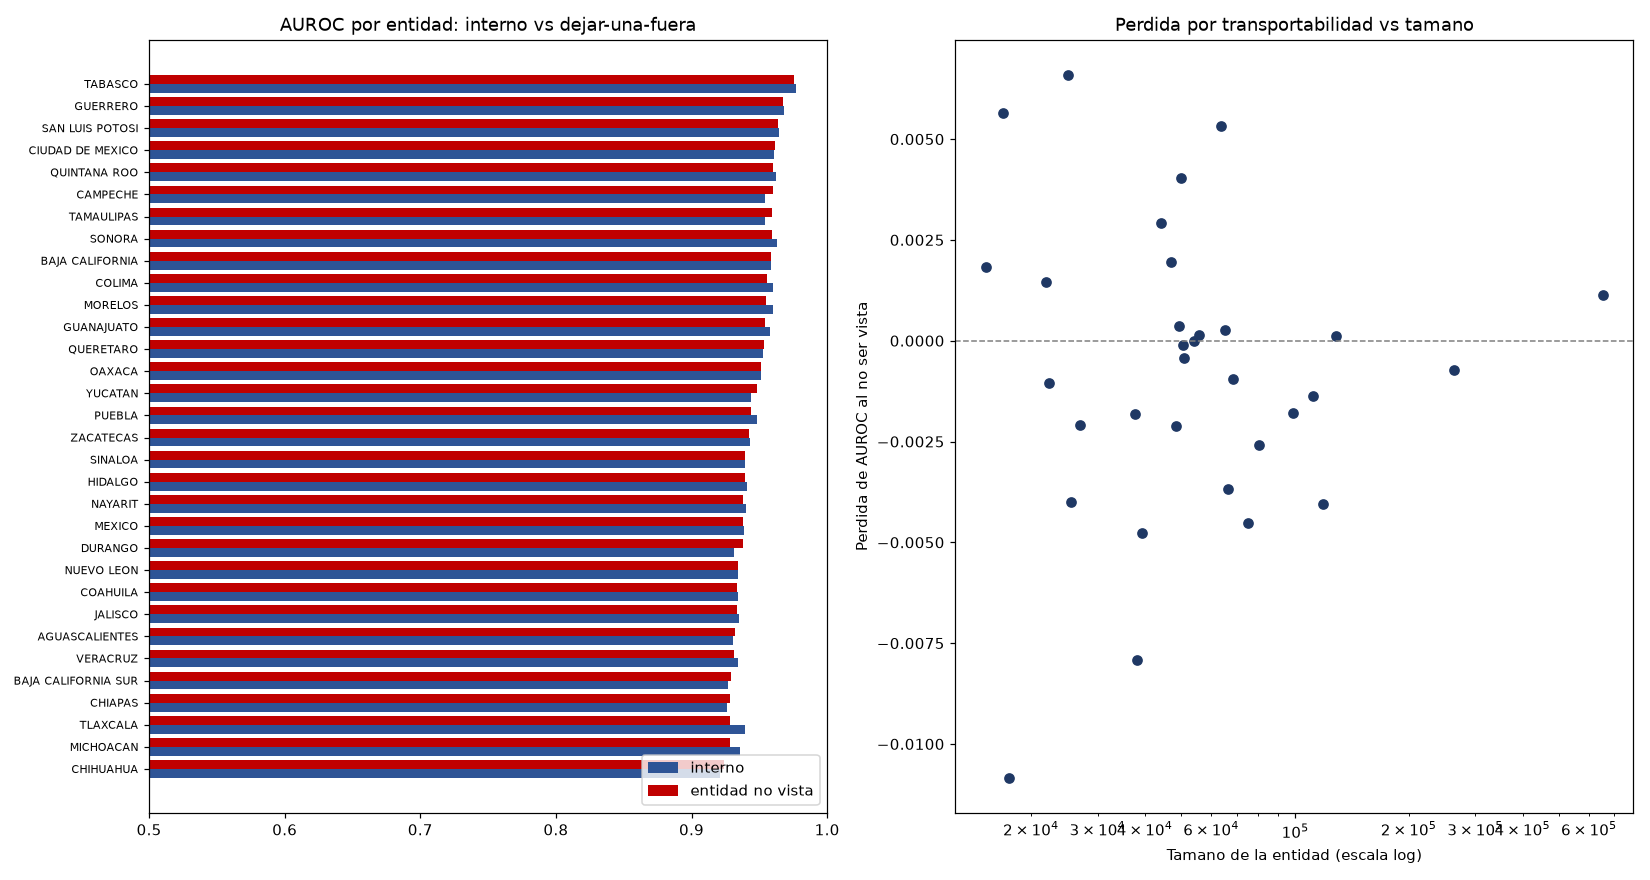
\includegraphics[width=\linewidth]{transportabilidad_loeo.png}
\caption{Transportabilidad geográfica interna. Izquierda: AUROC por entidad
habiendo participado en el entrenamiento frente a haber sido excluida.
Derecha: pérdida frente al tamaño de la entidad.}
\label{fig:loeo}
\end{figure}

\textbf{El desempeño se transfiere casi intacto.} La pérdida mediana de AUROC al
no haber visto la entidad es \loeoMediana, con un rango de $[\loeoMin,
\loeoMax]$: la entidad más afectada, \loeoPeor, pierde \loeoPeorDelta. De las
\loeoNent{} entidades, \loeoEmpeoran{} empeoran y el resto mejora; solo
\loeoMayoresUnPct{} supera una diferencia absoluta de 0.01.

\textbf{Las disparidades tampoco se acentúan.} La brecha de AUROC entre entidades
pasa de \loeoGapAurocInterno{} a \loeoGapAurocFuera{} y la de sensibilidad de
\loeoGapTprInterno{} a \loeoGapTprFuera: ambas se mantienen o se reducen
ligeramente.

El resultado tiene una lectura sustantiva que refuerza el argumento central. La
pérdida por transportabilidad no guarda relación con el tamaño de la entidad
($r=\loeoCorrTamr$, $p=\loeoCorrTamp$), de modo que el modelo no depende de haber
visto un estado concreto para funcionar en él. Combinado con el fracaso de la
reponderación (sección~\ref{sec:mitigacion_res}), esto cierra la explicación por
representación: la inequidad geográfica no proviene de que el modelo haya visto
pocos datos de ciertos estados --se comporta igual sin haber visto ninguno-- sino
de aplicar una regla de decisión común a poblaciones con distribuciones de riesgo
distintas.

La única asociación detectable es con la mortalidad de la entidad
($r=\loeoCorrTasar$, $p=\loeoCorrTasap$): los estados con más defunciones pierden
algo más al no haber sido vistos. Es la misma dirección que la correlación entre
AUROC y mortalidad de la sección~\ref{sec:correlatos}, y apunta al mismo
mecanismo pendiente de identificar.

\nota{Este diseño no sustituye a la validación externa. Que un modelo generalice
a un estado no visto \emph{de la misma fuente, el mismo año y el mismo proceso de
captura} dice poco sobre si generalizaría a otro sistema de registro. La
hipótesis~\ref{h4} sigue sin poner a prueba.}

\section{Mitigación de sesgo}
\label{sec:mitigacion_res}

La tabla~\ref{tab:mitigacion} compara las tres familias de intervención sobre el
mismo conjunto de prueba y el mismo punto de operación.

% Generado por generar_tablas.py -- NO editar a mano.

\begin{table}[htbp]
\centering
\caption{Comparación de las tres familias de mitigación sobre el conjunto de
prueba. Menor $\Delta$TPR indica mayor equidad entre entidades.}
\label{tab:mitigacion}
\small\setlength{\tabcolsep}{5pt}
\begin{tabular}{l r r r r}
\toprule
Intervención & $\Delta$TPR & $\Delta$FPR & Selec. & Exact.\ bal. \\
\midrule
Línea de base (umbral global) & 0.294 & 0.087 & 0.100 & 0.868 \\
Pre: reponderación por entidad & 0.290 & 0.082 & 0.099 & 0.865 \\
In: \emph{equalized odds} (Fairlearn)\textsuperscript{a} & 0.445 & -- & -- & -- \\
Post: umbral por entidad\textsuperscript{b} & 0.140 & 0.101 & 0.102 & 0.871 \\
Post: umbral por entidad (en muestra)\textsuperscript{c} & 0.022 & 0.107 & 0.101 & 0.869 \\
\bottomrule
\end{tabular}

\vspace{0.4em}
\begin{minipage}{0.95\linewidth}\footnotesize
\textsuperscript{a} Evaluado en una submuestra del bloque de entrenamiento
($n=\numprint{120000}$) y con un clasificador lineal; no es comparable uno a uno
con las demás filas. La reducción devuelve una distribución sobre clasificadores:
sobre 20 realizaciones del mismo modelo
ajustado, la brecha tiene mediana 0.397 y rango
[0.245, 0.628], intervalo
que contiene a la línea de base.\\
\textsuperscript{b} Umbrales estimados en el bloque de calibración y evaluados
en el de prueba: es la cifra desplegable.\\
\textsuperscript{c} Umbrales estimados sobre el propio conjunto de prueba:
cota optimista, reportada solo para dimensionar el sesgo de ajuste en muestra.
\end{minipage}
\end{table}


\subsection{Pre-procesamiento}

La reponderación inversa al tamaño de la entidad deja la brecha de sensibilidad
prácticamente intacta: \gapPre{} frente a \gapBase{} de la línea de base, con una
ligera pérdida de exactitud balanceada. El resultado es informativo: el problema
no es que el modelo haya visto pocos datos de las entidades pequeñas, sino que la
regla de decisión --un corte único-- interactúa mal con distribuciones de riesgo
heterogéneas. Reponderar la representación no puede corregir eso.

\subsection{In-procesamiento}

La reducción con restricción de \emph{equalized odds} arroja una brecha de
\gapIn, es decir, \emph{superior} a la de la línea de base. Pero el número
puntual no es lo relevante, y reportarlo solo sería engañoso.

La reducción por gradiente exponenciado no devuelve un clasificador, sino una
\emph{distribución} sobre clasificadores, de la que la predicción muestrea. Sobre
el mismo modelo ya ajustado y el mismo conjunto de evaluación,
\inRealizaciones{} realizaciones producen brechas con mediana \inMediana{} y
rango $[\inMin, \inMax]$. Ese intervalo contiene a la línea de base
(\gapBase) y es más ancho que cualquier efecto que pudiera atribuirse a la
restricción de equidad: la brecha depende más de qué realización toque que de la
intervención.

La interpretación correcta no es que el método sea inadecuado en general, sino
que resulta inestable en este régimen: con 32 grupos, algunos con pocos casos
positivos, el juego minimax que resuelve el algoritmo persigue la brecha máxima,
que en grupos pequeños está dominada por varianza de muestreo. A ello se suman las
limitaciones del montaje --submuestra y aprendiz lineal-- que impiden una
comparación uno a uno, como se advierte en la propia tabla.

\nota{Esta dispersión es también una advertencia de reproducibilidad. Si no se
fija la semilla en el momento de predecir --y no basta con fijarla al ajustar--,
el resultado del método cambia entre ejecuciones sin que nada lo señale. Un
trabajo que reportase una sola realización podría concluir tanto que la
intervención reduce la brecha como que la duplica.}

\subsection{Post-procesamiento}

El ajuste de umbrales por entidad es la única intervención efectiva. Con umbrales
estimados en el bloque de calibración y evaluados en el de prueba, la brecha de
sensibilidad cae de \gapBase{} a \gapPost, una reducción de \reduccionPost\,\%,
mientras la exactitud balanceada \emph{mejora} ligeramente, de \accBase{} a
\accPost, y la tasa de selección global se mantiene en torno a \selGlobal. Es decir: en
este problema la equidad geográfica se puede mejorar sustancialmente sin costo de
desempeño agregado.

\nota{La misma intervención, con umbrales estimados sobre el propio conjunto de
prueba, produce una brecha de \gapPostOpt. Esa cifra es una cota optimista y no
una política desplegable: mide qué tan bien se puede ajustar en retrospectiva, no
qué tan bien generalizaría. La diferencia entre \gapPostOpt{} y \gapPost{} --un
factor de \factorOptimismo-- dimensiona el sesgo que introduce estimar umbrales en
muestra, y es la razón por la que este trabajo reporta la segunda cifra como
resultado.}

\subsection{Frontera de Pareto}

La tabla~\ref{tab:pareto} y la figura~\ref{fig:pareto} presentan la frontera
obtenida interpolando entre el umbral global y los umbrales por entidad.

% Generado por generar_tablas.py -- NO editar a mano.

\begin{table}[htbp]
\centering
\caption{Frontera de Pareto equidad--desempeño. El parámetro $\alpha$ interpola
entre el umbral global ($\alpha=0$) y el umbral por entidad estimado fuera de
muestra ($\alpha=1$). Cada fila es una política de despliegue posible.}
\label{tab:pareto}
\begin{tabular}{r r r r}
\toprule
$\alpha$ & $\Delta$TPR & Exactitud balanceada & Selección \\
\midrule
0.0 & 0.2935 & 0.8680 & 0.1005 \\
0.1 & 0.2813 & 0.8672 & 0.0987 \\
0.2 & 0.2746 & 0.8664 & 0.0977 \\
0.3 & 0.2491 & 0.8667 & 0.0978 \\
0.4 & 0.2341 & 0.8693 & 0.0993 \\
0.5 & 0.2207 & 0.8713 & 0.1004 \\
0.6 & 0.2207 & 0.8706 & 0.0996 \\
0.7 & 0.2180 & 0.8700 & 0.0992 \\
0.8 & 0.2180 & 0.8703 & 0.0998 \\
0.9 & 0.1840 & 0.8695 & 0.0999 \\
1.0 & 0.1402 & 0.8711 & 0.1024 \\
\bottomrule
\end{tabular}
\end{table}


\begin{figure}[htbp]
\centering
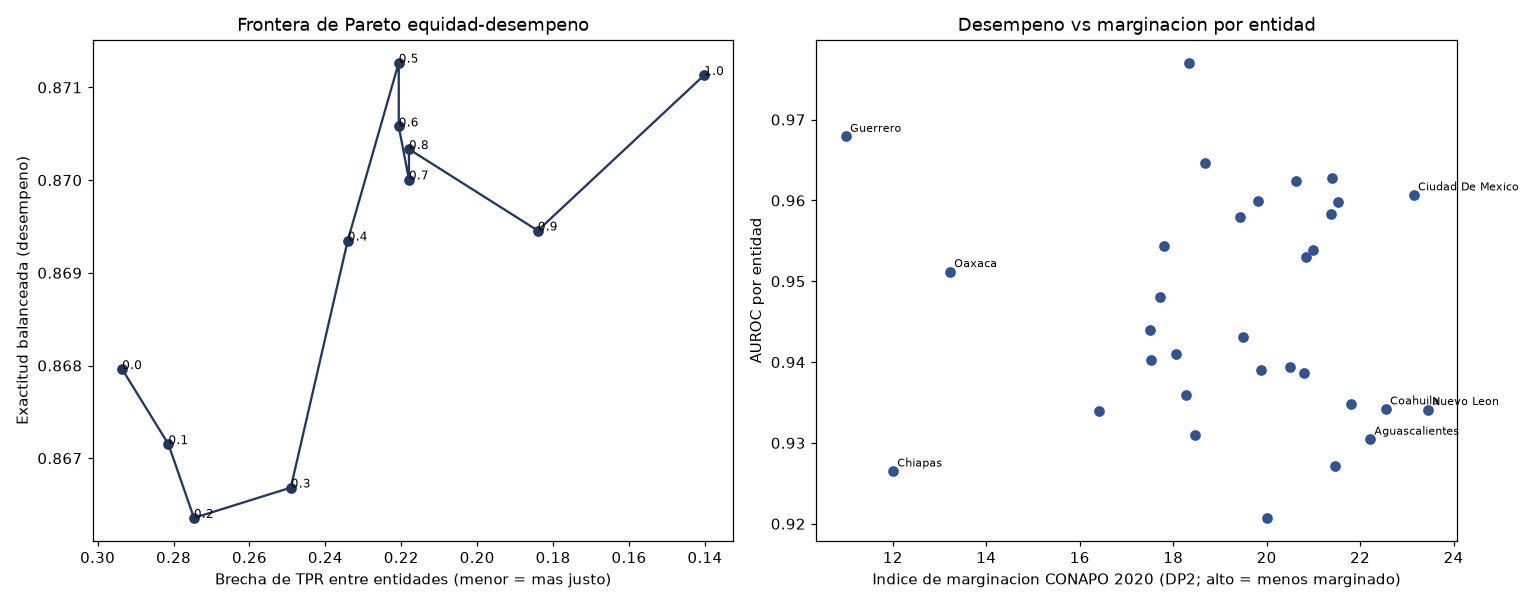
\includegraphics[width=\linewidth]{pareto_mitigacion.png}
\caption{Frontera de Pareto equidad--desempeño (izquierda) y desempeño por entidad
frente al índice de marginación de CONAPO 2020 (derecha; un valor más alto indica
menor marginación).}
\label{fig:pareto}
\end{figure}

La forma de la frontera es el resultado con mayor valor práctico: la exactitud
balanceada permanece en la banda \paretoAccMin--\paretoAccMax{} a lo largo de todo
el recorrido, mientras la brecha de sensibilidad desciende de \paretoGapMax{} a
\paretoGapMin. No hay, en este
problema, un intercambio material entre equidad y desempeño agregado; la
resistencia a corregir la disparidad no puede justificarse invocando pérdida de
utilidad clínica global.

Conviene señalar que el descenso no es monótono ni suave: entre $\alpha=0.5$ y
$\alpha=0.8$ la brecha se estanca en torno a
\paretoMesetaMin--\paretoMesetaMax. Ese estancamiento
refleja que la brecha máxima está determinada por unas pocas entidades extremas, y
que la interpolación lineal solo las alcanza cuando $\alpha$ se aproxima a 1.
Para el despliegue, la lectura es que las políticas intermedias rinden menos de lo
que sugeriría una interpolación proporcional.

\chapter{Discusión}
\label{cap:discusion}

\section{Evaluación de las hipótesis}

\subsection*{H1: disparidades entre entidades federativas}

\textbf{Sostenida.} Un modelo con AUROC de \aurocGlobal{} presenta una brecha de
sensibilidad de \gapTPRentidad{} y una brecha de AUROC de \gapAUROCentidad{} entre
entidades. La disparidad persiste al restringir el análisis a adultos de 60 años o
más, donde el rango de AUROC va de \sesentaPeorAUROC{} a \sesentaMejorAUROC, lo
que descarta que sea un reflejo de la composición etaria de los estados.

Resiste además dos pruebas de robustez que podrían haberla desmentido. En el
subconjunto hospitalizado --la población en la que el desenlace es posible-- no
solo persiste sino que la brecha de AUROC casi se triplica, hasta \hospGapAUROC{}
(sección~\ref{sec:sensibilidad_res}). Y no se debe a la composición del
entrenamiento: un modelo que nunca vio una entidad rinde en ella casi igual que
uno que sí la vio (sección~\ref{sec:loeo_res}).

La formulación original hablaba de disparidades «estadísticamente
significativas», y esa cualificación ahora sí puede sostenerse. Ninguna de las
\boP{} reasignaciones al azar de la etiqueta de entidad produjo una brecha tan
grande como la observada, ni en AUROC ni en sensibilidad ($p=\pAuroc$ y
$p=\pTpr$, el mínimo alcanzable con ese número de permutaciones), y
\paresPct\,\% de los pares de entidades tienen intervalos de AUROC disjuntos
(sección~\ref{sec:incertidumbre_res}).

El contraste obliga además a matizar la magnitud. La brecha nula no es cero: con
32 grupos desiguales, el azar produce una separación mediana de \nulaTpr{} en
sensibilidad. El exceso atribuible a la entidad es de unos \excesoTpr, no los
\gapTPRentidad{} completos. Sigue siendo una disparidad grande, pero conviene
reportarla contra la referencia correcta y no contra cero.

\subsection*{H2: asociación con la infraestructura o marginación}

\textbf{No sostenida.} El índice de marginación de CONAPO 2020 no muestra
asociación detectable con el desempeño por entidad ($r=\corrMargAurocr$,
$p=\corrMargAurocp$), y el resultado se sostiene al agregar por grado de
marginación, donde una prueba de Kruskal--Wallis tampoco detecta diferencia
($H=\kruskalH$, $p=\kruskalP$). El grupo con menor AUROC medio es, de hecho, el
de marginación \emph{muy baja}: si hay una tendencia, apunta en dirección
opuesta a la hipótesis.

Cabe una advertencia sobre el alcance de esta conclusión. La ausencia de
asociación con un índice compuesto no equivale a ausencia de mecanismo
estructural: la marginación socioeconómica agregada por entidad es un
\emph{proxy} grueso de lo que importaría aquí, que es la capacidad de registro y
atención de las unidades médicas. \ref{h2} queda refutada en la forma en que se
operacionalizó, no en su intuición de fondo.

El único correlato que alcanza significación convencional es la tasa de mortalidad
de la entidad ($r=\corrAurocTasar$, $p=\corrAurocTasap$): el modelo discrimina
peor donde más gente muere. Conviene no sobrevalorarlo: se examinaron tres
características por dos métricas y dos estadísticos, de modo que un único
$p$ apenas por debajo de 0.05 en una docena de contrastes no sobrevive a ninguna
corrección por multiplicidad. Se reporta como señal a investigar, no como
hallazgo confirmatorio. Esta asociación admite al menos dos lecturas que el diseño actual no puede
separar. Puede reflejar un mecanismo de \emph{atención}: en entidades con sistemas
más presionados, la muerte depende más de factores no capturados por el modelo
--disponibilidad de cama, oportunidad del traslado, saturación-- y menos del perfil
clínico inicial, de modo que hay un techo real a lo que la edad y las
comorbilidades pueden predecir. Y puede reflejar un mecanismo de \emph{registro}:
una mortalidad observada más alta puede indicar subdetección de casos leves, lo que
cambia la composición de la cohorte y con ella la dificultad de la tarea.
Distinguir ambas requiere indicadores de infraestructura por unidad médica, no por
entidad.

\subsection*{H3: mitigación con pérdida acotada de desempeño}

\textbf{Sostenida, con una precisión importante.} El post-procesamiento por
umbrales de entidad reduce la brecha de sensibilidad de \gapBase{} a \gapPost{}
--\reduccionPost\,\%-- sin pérdida de desempeño agregado: la exactitud balanceada
pasa de \accBase{} a \accPost. La frontera de Pareto muestra que el desempeño se
mantiene en la banda \paretoAccMin--\paretoAccMax{} en todo su recorrido, de modo que la pérdida es
inferior a cualquier umbral razonable que se hubiera fijado de antemano.

Hay, sin embargo, un costo que la exactitud balanceada no captura y que conviene
enunciar: al igualar la sensibilidad entre entidades, la brecha de \emph{tasa de
falsos positivos} empeora, de \postGapFPRbase{} a \postGapFPR. No es un defecto
del método sino exactamente lo que predice el teorema de imposibilidad
(capítulo~\ref{cap:marco}): con prevalencias distintas entre grupos, igualar una
de las dos tasas de \emph{equalized odds} desiguala la otra. Lo que el
post-procesamiento hace no es eliminar la inequidad, sino \emph{elegir} cuál de
las dos se reparte por igual --y elegir la sensibilidad, en un instrumento cuyo
costo de omitir una defunción excede al de una alarma innecesaria, es defendible.
Pero es una elección normativa que debe declararse, no un óptimo técnico.

La segunda precisión es que la mitigación \emph{no elimina} la disparidad. Una
brecha residual de \gapPost{} sigue siendo clínicamente relevante. Y el hallazgo
metodológico que acompaña al resultado es que la cifra de eliminación casi total
que se obtiene ajustando umbrales sobre el propio conjunto de prueba
(\gapPostOpt) es un artefacto de ajuste en muestra. Un trabajo que no separase el
bloque de calibración concluiría que el problema queda resuelto, cuando la brecha
desplegable es \factorOptimismo{} veces mayor.

\subsection*{H4: transportabilidad a una fuente independiente}

\textbf{Sin poner a prueba, con evidencia parcial en la dirección contraria a lo
esperado.} La validación externa en la base de Egresos Hospitalarios de la DGIS no
se ha ejecutado, de modo que \ref{h4} tal como está redactada --transferencia a
una \emph{fuente independiente}-- no queda ni sostenida ni refutada.

Sí se puso a prueba la generalización geográfica dentro de la misma fuente
(sección~\ref{sec:loeo_res}), y el resultado va en contra de lo que \ref{h4}
anticipaba: al excluir por completo una entidad del entrenamiento, el desempeño
sobre ella apenas cambia (pérdida mediana \loeoMediana) y las disparidades no se
acentúan, sino que se mantienen o se reducen. Esto acota la hipótesis: si las
disparidades llegaran a agravarse en la base DGIS, no sería por no haber visto la
entidad, sino por el cambio de fuente, de definición de caso o de periodo.

La ejecución futura de \ref{h4} tiene además un prerrequisito que este trabajo
identificó y conviene dejar escrito. SAEH es una base de \emph{egresos}: su
población son pacientes hospitalizados, con una prevalencia del desenlace cercana
a \hospPrev{} frente a \cohorteTasaDef\,\% en esta cohorte. Aplicar sobre ella el
modelo principal produciría una caída de desempeño atribuible al cambio de
espectro y no a la transportabilidad. La validación externa debe hacerse con el
modelo restringido a hospitalizados de la sección~\ref{sec:sensibilidad_res}, no
con el de la cohorte completa.

\section{Asimetría entre familias de mitigación}

El resultado comparativo tiene, a nuestro juicio, valor propio. Las tres familias
de mitigación se presentan habitualmente como alternativas de eficacia
comparable, a elegir según restricciones operativas. En este problema la
diferencia es cualitativa: el pre-procesamiento no mueve la brecha, el
in-procesamiento arroja un resultado tan disperso que no permite concluir nada
--su rango entre realizaciones, $[\inMin, \inMax]$, contiene a la línea de
base-- y solo el post-procesamiento la reduce, a la mitad y sin costo agregado.

La explicación está en la naturaleza del sesgo. La disparidad no proviene de un
ordenamiento defectuoso: el AUROC por entidad es alto en todas
(\entPeorAUROC--\entMejorAUROC), y el modelo está bien calibrado en cada una
(error máximo \errCalEntidad). Proviene de aplicar un \emph{corte único} a
distribuciones de riesgo que difieren entre entidades. Cuando el defecto está en
la regla de decisión y no en la función de puntuación, la intervención que corrige
la regla de decisión es la que funciona. Reponderar los datos de entrenamiento
ataca un problema de representación que aquí no es el que causa la brecha.

Esto sugiere una heurística transferible: antes de elegir la familia de
mitigación, conviene diagnosticar si la inequidad reside en el ordenamiento
--brechas de AUROC grandes-- o en el umbral --AUROC similar con brechas de TPR
grandes. Aquí la brecha de sensibilidad (\gapTPRentidad) es \razonBrechas{} veces
la de AUROC (\gapAUROCentidad), lo que apuntaba al umbral desde el diagnóstico.
Ese diagnóstico, sin embargo, es específico de la cohorte completa. Entre los
pacientes hospitalizados la relación se invierte --la brecha de AUROC sube a
\hospGapAUROC{} y la de sensibilidad baja a \hospGapTPR-- y en el subgrupo de 60
años o más la dispersión del AUROC llega a \sesentaRango. La heurística, por
tanto, no es «diagnostíquese una vez», sino «diagnostíquese en la población sobre
la que se va a desplegar»: en la población en riesgo, una mitigación basada solo
en umbrales sería insuficiente.

\section{Implicaciones para el despliegue}

\begin{enumerate}[leftmargin=*]
  \item \textbf{Un umbral nacional único no es una decisión neutral.} Es una
    decisión que redistribuye sensibilidad entre entidades. Conviene precisar en qué
    dirección: la sensibilidad por entidad \emph{no} está asociada a su mortalidad
    ($r=\corrTprTasar$, $p=\corrTprTasap$), de modo que el reparto no penaliza
    sistemáticamente a los estados con más defunciones; lo que sí decae en ellos es
    la discriminación ($r=\corrAurocTasar$, $p=\corrAurocTasap$). La inequidad de
    sensibilidad no sigue un eje interpretable, y eso la hace más difícil de
    justificar, no menos: la neutralidad aparente de «el mismo umbral para todos»
    reparte la protección de forma esencialmente arbitraria entre estados.
  \item \textbf{La frontera de Pareto es el entregable adecuado para el
    regulador.} La elección de $\alpha$ es normativa. El análisis técnico puede
    mostrar que no cuesta desempeño agregado; no puede decidir cuánta
    diferenciación por entidad es aceptable en términos de equidad horizontal
    entre ciudadanos.
  \item \textbf{Umbrales por entidad plantean una objeción legítima.} Usar la
    residencia en el momento de la decisión implica tratar de forma distinta a dos
    pacientes con idéntico perfil clínico. La justificación es que el trato
    formalmente idéntico ya produce resultados desiguales; pero es un argumento que
    debe hacerse explícito ante un comité de ética, no asumirse.
  \item \textbf{La calibración debe verificarse antes de auditar equidad.} Como
    muestra el capítulo~\ref{cap:resultados}, auditar sobre puntajes descalibrados
    habría producido una conclusión invertida sobre la calibración por grupo.
  \item \textbf{Humano en el circuito.} Con una tasa de selección de \selGlobal{} y un
    valor predictivo positivo modesto en el punto de operación, el instrumento es
    de priorización y no de decisión automatizada.
\end{enumerate}

\section{Relación con la literatura}

El modelo de referencia coincide con la literatura sobre esta
base~\parencite{becerra2022,mendez2024} en las variables que resultan más
informativas --neumonía y edad-- lo que respalda que el sujeto de la auditoría sea
representativo y no un modelo debilitado. Una comparación numérica directa del
desempeño no es posible, porque esos trabajos reportan exactitud y $F_1$ sobre
umbrales no declarados y esta tesis reporta AUROC y sensibilidad en un punto de
operación explícito.

Respecto del trabajo que estudia los factores geográficos como
predictores~\parencite{geograficos2024}, los resultados de esta tesis son
complementarios y no contradictorios. Que la entidad sea informativa como
predictor y que el modelo sea desigualmente preciso entre entidades son hechos
distintos; el segundo es el que importa para el despliegue responsable, y es el
que no se había medido. Es de notar que el modelo auditado aquí \emph{no} usa la
entidad como predictor, y aun así su desempeño depende de ella: la inequidad
geográfica no requiere que la geografía entre al modelo.

Frente a la literatura de equidad en salud anclada en otros
contextos~\parencite{nejadshamsi2026,riccilara2022}, la aportación es el traslado del
marco a un atributo sensible --la entidad federativa-- con significado
institucional propio en México, donde la desigualdad entre estados es un rasgo
estructural del sistema y no una variable de composición poblacional. Que el
índice de marginación no explique la brecha no debilita esa elección: confirma
que la entidad captura algo que los agregados socioeconómicos estatales no
miden, y esa es precisamente la razón para auditarla como atributo propio.

\section{Limitaciones}
\label{sec:limitaciones}

\begin{enumerate}[leftmargin=*]
  \item \textbf{Sin validación externa.} Todo el análisis vive en una fuente y un
    año. La generalización geográfica interna sí se evaluó
    (sección~\ref{sec:loeo_res}) y resultó buena, pero no sustituye a una segunda
    fuente.
  \item \textbf{El desenlace vive en el \fracHosp\,\% de la cohorte.} Fallecer
    implica estar registrado como hospitalizado, de modo que parte de la
    discriminación del modelo principal es separar ambulatorios de hospitalizados.
    Las cifras comparables con modelos clínicos de mortalidad son las de la
    sección~\ref{sec:sensibilidad_res}, no las de la cohorte completa.
  \item \textbf{Incertidumbre acotada solo en el eje principal.} La auditoría
    por entidad se acompaña de intervalos de confianza y prueba de permutación,
    pero los subgrupos interseccionales y los ejes de sexo y edad se reportan como
    estimaciones puntuales. El ordenamiento fino de la tabla~\ref{tab:entidad}
    tampoco debe leerse posición por posición: solo \paresPct\,\% de los pares
    tienen intervalos disjuntos.
  \item \textbf{Marginación medida a escala estatal.} El índice de CONAPO está
    verificado, pero agrega condiciones socioeconómicas por entidad. El mecanismo
    que \ref{h2} postula --capacidad de atención-- opera a escala de unidad médica,
    de modo que la ausencia de asociación acota la hipótesis pero no la cierra.
  \item \textbf{Un solo año y un solo desenlace.} No se modela hospitalización ni
    se evalúa estabilidad temporal entre olas epidémicas, cuya composición de casos
    y presión hospitalaria difieren de forma conocida.
  \item \textbf{Sesgo de verificación en la cohorte.} Restringir a casos
    confirmados condiciona a haber sido detectado y probado, y la propensión a
    detectar varía entre entidades. Parte de la disparidad observada puede
    originarse en el proceso de captura y no en el modelo. Este es, a nuestro
    juicio, el supuesto más frágil del diseño y no puede corregirse dentro de esta
    fuente.
  \item \textbf{Dependencia de una variable.} Con \texttt{NEUMONIA} concentrando
    la importancia, un cambio en la práctica de registro entre entidades se
    traduciría directamente en desempeño desigual. Falta el análisis de
    sensibilidad que lo descarte.
  \item \textbf{Validación por partición aleatoria.} No se realizó validación
    temporal ni dejando-una-entidad-fuera, que es el diseño natural para evaluar
    generalización geográfica.
\end{enumerate}

\chapter{Conclusiones y trabajo futuro}
\label{cap:conclusiones}

\section{Conclusiones}

Esta tesis partió de una premisa que la literatura respalda: predecir mortalidad
por COVID-19 con datos abiertos mexicanos es un problema resuelto. Sobre esa base
desplazó la pregunta de si el modelo acierta a si acierta por igual, tomando la
entidad federativa como atributo sensible. Las conclusiones son cinco.

\textbf{Primera: la inequidad geográfica existe y es sustantiva.} Un modelo con
AUROC de \aurocGlobal{} reparte su sensibilidad de forma muy desigual entre
estados: la brecha es \gapTPRentidad{} en un punto de operación calibrado para
detectar el \sensObjetivo\,\% de las defunciones a escala nacional. Traducido, el
modelo detecta cerca de \entPeorPct{} de cada 100 defunciones en la entidad peor
servida frente a \entMejorPct{} en la mejor. La disparidad es estadísticamente
significativa ($p=\pTpr$ frente a la nula por permutación), aunque conviene
descontar lo que el azar aporta con 32 grupos desiguales: el exceso atribuible a
la entidad es de unos \excesoTpr. Y ocurre \emph{sin} que la entidad sea un
predictor del modelo, lo que descarta la solución ingenua de «no usar la
geografía».

\textbf{Segunda: no se explica por composición demográfica.} Al restringir el
análisis a adultos de 60 años o más, la brecha no solo persiste sino que se
amplía. La inequidad es una propiedad del modelo operando sobre poblaciones
heterogéneas, no un artefacto de la estructura de edades de cada estado.

\textbf{Tercera: en la población completa la disparidad reside en el umbral, no
en el ordenamiento, y eso determina qué mitigación funciona.} El AUROC por entidad
es alto en todas y la calibración por entidad es buena (error máximo
\errCalEntidad); lo que falla es aplicar un corte único a distribuciones de riesgo
distintas. La salvedad importa: entre los pacientes hospitalizados --la población
donde el desenlace es posible-- la relación se invierte, con la brecha de AUROC en
\hospGapAUROC{} y la de sensibilidad en \hospGapTPR, y en el subgrupo de 60 años o
más la dispersión del AUROC llega a \sesentaRango. El diagnóstico, y con él la
elección de mitigación, debe hacerse sobre la población en la que se desplegará. Por eso la
reponderación previa al entrenamiento no cambia nada, la restricción de
\emph{equalized odds} durante el entrenamiento resulta inestable con 32 grupos
desiguales, y solo el ajuste de umbrales por entidad reduce la brecha --de
\gapBase{} a \gapPost, un \reduccionPost\,\%-- y lo hace \emph{sin} costo de
desempeño agregado (exactitud balanceada de \accBase{} a \accPost). El costo está
en otra parte y es el que predice la teoría: al igualar la sensibilidad, la brecha
de falsos positivos crece de \postGapFPRbase{} a \postGapFPR. La mitigación no
elimina la inequidad; elige cuál de las dos tasas se reparte por igual. La
recomendación práctica que se desprende es diagnosticar primero dónde vive el
sesgo --brechas de AUROC frente a brechas de sensibilidad-- y elegir la familia de
mitigación en consecuencia.

\textbf{Cuarta: la inequidad no es un problema de cobertura de datos.} Al excluir
por completo una entidad del entrenamiento y evaluar sobre ella, el desempeño
apenas se mueve --pérdida mediana de AUROC \loeoMediana{} sobre \loeoNent{}
entidades-- y las brechas no se acentúan. La pérdida además no guarda relación con
el tamaño de la entidad ($r=\loeoCorrTamr$, $p=\loeoCorrTamp$). Junto con el
fracaso de la reponderación, esto descarta la explicación más intuitiva: el modelo
no falla en unos estados por haber visto pocos datos suyos; funciona igual sin
haber visto ninguno. Tampoco es un efecto de la práctica de registro de la
variable dominante: al reentrenar sin \texttt{\impPrimeraVar} la brecha de AUROC
no se reduce, sino que sube a \sinNeuGapAUROC. Lo que produce la inequidad es
aplicar una regla común a poblaciones distintas.

\textbf{Quinta: la separación metodológica no es un detalle.} Dos decisiones de
diseño cambian conclusiones sustantivas. Auditar la calibración por grupo sobre
puntajes sin calibrar habría reportado un error de \errCalCrudo{} y una conclusión de
«calibración inequitativa» que corresponde en realidad al sesgo global de
entrenamiento; medido sobre riesgo calibrado, el error es \errCalEntidad{} y la
calibración por entidad es buena. Y estimar los umbrales de mitigación sobre el
propio conjunto de prueba habría llevado a declarar la brecha prácticamente
eliminada (\gapPostOpt) cuando la cifra desplegable es \gapPost, \factorOptimismo{} veces
mayor.

Estas conclusiones se sostienen dentro de los límites declarados en la
sección~\ref{sec:alcance} y con las limitaciones de la
sección~\ref{sec:limitaciones}. En particular, la hipótesis~\ref{h2} queda
refutada en la forma en que se operacionalizó --el índice de marginación estatal
no predice el sesgo-- y la hipótesis~\ref{h4} sin poner a prueba, si bien la
generalización geográfica interna, que es lo más cercano que puede evaluarse sin
una segunda fuente, resultó buena.

\section{Trabajo futuro}
\label{sec:trabajo_futuro}

Ordenado por prioridad, entendida como la capacidad de cada tarea para modificar
las conclusiones anteriores:

\begin{enumerate}[leftmargin=*]
  \item \textbf{Extender la cuantificación de incertidumbre.} El eje geográfico
    ya cuenta con intervalos de confianza y prueba de permutación
    (sección~\ref{sec:incertidumbre_res}); falta hacer lo propio con los subgrupos
    interseccionales, donde los tamaños son mucho menores y la precisión es la
    principal duda abierta.
  \item \textbf{Indicadores de infraestructura de salud.} El índice de
    marginación de CONAPO ya está incorporado y no explica el sesgo. El paso
    siguiente es sustituirlo por el mecanismo que \ref{h2} postula en realidad:
    camas, personal y equipamiento por habitante, idealmente por unidad médica y
    no por entidad.
  \item \textbf{Validación externa en la base DGIS.} Es el paso que pone a prueba
    \ref{h4} y el que la literatura casi nunca da. Tiene un prerrequisito que este
    trabajo dejó identificado: SAEH es una base de egresos y su población son
    pacientes hospitalizados, con una prevalencia del desenlace cercana a
    \hospPrev{} frente a \cohorteTasaDef\,\% aquí. Debe validarse el modelo
    restringido a hospitalizados (sección~\ref{sec:sensibilidad_res}); usar el de la
    cohorte completa haría pasar un cambio de espectro por un fallo de
    transportabilidad. Requiere además reconstruir las once comorbilidades desde
    los códigos CIE-10 de SAEH, lo que añade desplazamiento de medición al de
    población.
  \item \textbf{Validación temporal.} Dividir por olas epidémicas y entrenar en un
    año para evaluar en otro, con los cortes anuales de la DGE. La generalización
    geográfica ya se evaluó (sección~\ref{sec:loeo_res}); la temporal no.
  \item \textbf{Umbrales por grupo con regularización.} Contraer los umbrales de
    entidades pequeñas hacia el umbral global, en lugar de estimarlos de forma
    independiente. Es la vía natural para atacar la brecha residual de \gapPost{}
    sin perseguir ruido.
  \item \textbf{Sesgo de verificación.} Modelar explícitamente la propensión a la
    detección por entidad, para separar la inequidad del modelo de la inequidad del
    proceso de captura.
  \item \textbf{Desenlace de hospitalización y utilidad clínica.} Extender el
    análisis al segundo desenlace y añadir análisis de curva de decisión
    (\emph{net benefit})~\parencite{vickers2006} y explicaciones locales, previstos en
    el protocolo y no ejecutados.
\end{enumerate}


% \raggedright dentro de un grupo: los DOI largos no se pueden dividir y
% justificados desbordan el margen.
\begingroup
\raggedright
\printbibliography[heading=bibintoc,title={Referencias}]
\endgroup

\appendix
\chapter{Reproducibilidad del canal analítico}
\label{ap:reproducibilidad}

\section{Estructura y orden de ejecución}

El análisis se implementa en seis cuadernos de Jupyter que deben ejecutarse en
orden, más un módulo compartido que fija el contrato entre ellos:

\begin{table}[htbp]
\centering
\caption{Artefactos del canal analítico.}
\label{tab:artefactos}
\small
\setlength{\tabcolsep}{4pt}
\begin{tabular}{p{3.9cm} p{5.4cm} p{4.4cm}}
\toprule
Componente & Función & Salidas \\
\midrule
\texttt{tesis\_common.py} &
Contrato compartido: rutas, cohorte, hiperparámetros, partición, punto de
operación y métricas de equidad & --- \\
\texttt{01\_exploracion\allowbreak\_datos\_dge} &
Ingesta, recodificación, control de fuga, análisis exploratorio &
\texttt{*.parquet}, \texttt{*.manifest.json}, \texttt{calidad\allowbreak\_datos.json},
figura del EDA \\
\texttt{02\_modelo\_referencia} &
Entrenamiento, calibración isotónica, punto de operación, importancia y
sensibilidad al subconjunto hospitalizado y a la exclusión de
\texttt{NEUMONIA} &
\texttt{modelo\_hgb\allowbreak\_mortalidad\allowbreak.joblib},
\texttt{modelo\allowbreak\_referencia.json},
\texttt{sensibilidad\allowbreak\_hospitalizados.json} \\
\texttt{03\_auditoria\_equidad} &
Auditoría por entidad, sexo, edad e interseccional &
\texttt{auditoria\allowbreak\_equidad.json}, figura de equidad \\
\texttt{04\_mitigacion\_pareto} &
Correlatos, tres familias de mitigación, frontera de Pareto &
\texttt{resultados\allowbreak\_tesis.json}, figura de Pareto \\
\texttt{05\_transportabilidad\allowbreak\_loeo} &
Dejar-una-entidad-fuera: \loeoNent{} modelos, cada uno excluyendo una entidad &
\texttt{transportabilidad\allowbreak\_loeo.json}, figura de transportabilidad \\
\texttt{06\_incertidumbre} &
Remuestreo (\boB{} réplicas) y prueba de permutación (\boP) sobre las brechas &
\texttt{incertidumbre\allowbreak\_brechas.json}, figura de incertidumbre \\
\texttt{generar\_tablas.py} &
Traduce los JSON a tablas y macros de \LaTeX{} &
\texttt{tesis/tablas/}, \texttt{macros\allowbreak\_resultados.tex} \\
\bottomrule
\end{tabular}
\end{table}

\section{Contrato de datos entre etapas}

El riesgo característico de un canal por cuadernos es que una etapa consuma un
artefacto producido por una versión anterior de la etapa previa, sin que nada lo
señale. Para evitarlo, cada etapa verifica la procedencia de lo que consume antes
de usarlo:

\begin{enumerate}[leftmargin=*]
  \item El cuaderno 01 escribe, junto al conjunto de datos limpio, un
    \textbf{manifiesto} en JSON con la cohorte empleada, el número de filas, la
    lista de columnas, las tasas de desenlace y las versiones de biblioteca.
  \item Los cuadernos 02 a 04 llaman a \texttt{cargar\_cohorte()}, que exige la
    presencia del manifiesto y verifica columnas requeridas, número de filas y
    bandera de cohorte. Cualquier discrepancia detiene la ejecución con un mensaje
    accionable en lugar de continuar.
  \item El modelo se persiste como \textbf{paquete} --estimador, calibrador,
    lista de predictores, hiperparámetros y huella de la cohorte-- y no como
    estimador desnudo. \texttt{cargar\_modelo()} rechaza un modelo entrenado sobre
    otra cohorte o con otros predictores.
  \item La escritura del conjunto limpio \textbf{falla de inmediato} si no puede
    completarse, en lugar de degradar a otro formato: una degradación silenciosa
    dejaría en disco el artefacto de la corrida anterior.
\end{enumerate}

El cuaderno 05 es la única excepción deliberada a la regla de que solo el 02
entrena: su objeto de estudio \emph{es} un conjunto de modelos que nunca vieron la
entidad evaluada. El 06 no entrena: reconstruye el escenario auditado y solo
remuestrea sobre él. Usa los hiperparámetros canónicos, de modo que la única
diferencia con la línea de base es qué entidades entraron al ajuste.

Los hiperparámetros del modelo, la partición, el punto de operación, los cortes de
edad y las métricas de equidad tienen una única definición, en
\texttt{tesis\_common.py}. Ninguna etapa los redefine, de modo que la alineación
entre cuadernos es estructural y no depende de que coincidan por convención.

\section{Determinismo}

Todas las operaciones estocásticas usan semilla fija (42, salvo la submuestra del
método de in-procesamiento, que usa 3). La partición se deriva de índices
posicionales estratificados por el desenlace, de modo que los bloques de
entrenamiento, calibración y prueba son idénticos en los cuadernos 02, 03 y 04.

Un caso merece mención aparte porque no se resuelve fijando la semilla del ajuste.
La reducción por gradiente exponenciado de Fairlearn devuelve una distribución
sobre clasificadores, y su método de predicción \emph{muestrea} de ella: sin una
semilla en la llamada a predecir, la misma ejecución sobre el mismo modelo ya
ajustado produce brechas distintas. Al detectarlo se midió el efecto --brechas
entre \inMin{} y \inMax{} sobre \inRealizaciones{} realizaciones-- y se fijó la
semilla también en la predicción. Sin esa corrección, el resultado del método de
in-procesamiento no era reproducible entre ejecuciones.

\section{Entorno de ejecución}

\begin{table}[htbp]
\centering
\caption{Versiones utilizadas para producir los resultados de este documento.}
\label{tab:entorno}
\small
\begin{tabular}{l l l l}
\toprule
Componente & Versión & Componente & Versión \\
\midrule
Python        & 3.14.5  & \texttt{scipy}       & 1.18.0 \\
\texttt{numpy}        & 2.5.1   & \texttt{fairlearn}   & 0.14.0 \\
\texttt{pandas}       & 3.0.5   & \texttt{matplotlib}  & 3.11.1 \\
\texttt{scikit-learn} & 1.9.0   & \texttt{joblib}      & 1.5.3 \\
\texttt{pyarrow}      & 25.0.0  & \TeX{} Live          & 2026 \\
\bottomrule
\end{tabular}
\end{table}

\section{Reproducción del documento}

\begin{enumerate}[leftmargin=*]
  \item Colocar el corte anual \texttt{\cohorteFuente} en el directorio raíz, o
    apuntar a él con la variable de entorno \texttt{DGE\_DATA\_PATH}.
  \item Ejecutar los seis cuadernos en orden.
  \item Ejecutar \texttt{python3 generar\_tablas.py} para regenerar tablas y
    macros.
  \item Compilar con \texttt{latexmk -pdf tesis.tex} desde el directorio
    \texttt{tesis/}.
\end{enumerate}

Las cifras del capítulo~\ref{cap:resultados} no se editan a mano en ningún punto:
provienen de macros generadas desde los archivos de resultados. Si una cifra del
texto no coincide con los cuadernos, es porque el paso 3 no se ejecutó, no porque
el texto y el análisis discrepen.

\chapter{Variables y codificación}
\label{ap:variables}

\section{Codificación de la fuente}

La base de la DGE codifica las variables categóricas con enteros y reserva valores
especiales para la ausencia de dato:

\begin{table}[htbp]
\centering
\caption{Códigos de la fuente relevantes para este trabajo.}
\label{tab:codigos}
\small
\begin{tabular}{l p{10.2cm}}
\toprule
Variable & Codificación \\
\midrule
Comorbilidades y signos & $1=$ sí; $2=$ no; $97=$ no aplica; $98=$ se ignora; $99=$ no especificado \\
\texttt{SEXO} & $1=$ mujer; $2=$ hombre; $99=$ no especificado \\
\texttt{TIPO\_PACIENTE} & $1=$ ambulatorio; $2=$ hospitalizado; $99=$ no especificado \\
\texttt{FECHA\_DEF} & Fecha de defunción; \texttt{9999-99-99} indica paciente vivo \\
\texttt{CLASIFICACION\_FINAL} & $1,2,3=$ caso COVID confirmado; $6=$ sospechoso; $7=$ negativo \\
\texttt{ENTIDAD\_RES} & $1$--$32$ entidades federativas; $97$--$99$ desconocido \\
\bottomrule
\end{tabular}
\end{table}

\section{Variables derivadas}

\begin{table}[htbp]
\centering
\caption{Variables construidas y su papel en el análisis.}
\label{tab:derivadas}
\small
\setlength{\tabcolsep}{4pt}
\begin{tabular}{p{3.5cm} p{3.2cm} p{7.4cm}}
\toprule
Variable & Papel & Definición \\
\midrule
\texttt{defuncion} & Desenlace &
$1$ si \texttt{FECHA\_DEF} $\neq$ \texttt{9999-99-99} \\
\texttt{hospitalizado} & Desenlace (no modelado) &
$1$ si \texttt{TIPO\_PACIENTE} $=2$ \\
\texttt{EDAD} & Predictor &
Valores fuera de $[0,120]$ marcados como faltantes \\
\texttt{sexo\_mujer} & Predictor y atributo sensible &
$1=$ mujer, $0=$ hombre, faltante si $99$ \\
\texttt{<comorbilidad>\_bin} & Predictor &
$1$ si el código es $1$; $0$ si es $2$; faltante en otro caso \\
\texttt{<comorbilidad>\_na} & Indicador de calidad &
$1$ si el código original es $97$, $98$ o $99$ \\
\texttt{entidad\_nombre} & Atributo sensible &
Nombre de la entidad de residencia; eje central de la auditoría \\
\texttt{grupo\_edad} & Atributo sensible &
Cortes 0--17, 18--39, 40--59, 60 o más \\
\bottomrule
\end{tabular}
\end{table}

\section{Predictores admitidos y variables excluidas}

Los trece predictores del modelo son la edad, el indicador de sexo y las once
comorbilidades binarizadas: diabetes, EPOC, asma, inmunosupresión, hipertensión,
otra comorbilidad, enfermedad cardiovascular, obesidad, enfermedad renal crónica,
tabaquismo y neumonía.

Quedan excluidas por posterioridad al punto de predicción, y por tanto por riesgo
de fuga de información: \texttt{UCI}, \texttt{INTUBADO} y \texttt{FECHA\_DEF}
--salvo como origen del desenlace-- así como \texttt{TIPO\_PACIENTE} en su papel de
predictor de mortalidad. La entidad de residencia y el grupo etario se excluyen
por una razón distinta: se reservan como atributos sensibles para la auditoría, no
por fuga.

Los indicadores \texttt{\_na} no se emplean como predictores en el modelo
reportado, pero se conservan en el conjunto de datos porque el dato faltante
resulta informativo y su frecuencia difiere entre entidades por un margen amplio
--de \naEntMin\,\% a \naEntMax\,\%--, lo que constituye un mecanismo plausible de
inequidad. El capítulo~\ref{cap:resultados} lo documenta; explotarlo o corregirlo
queda como trabajo futuro.


\end{document}
